% !TEX root = ../swarthmore_talk.tex

% Hilbert's 10 Problem
\begin{frame}[plain]
\frametitle{\textcolor{white}{Hilbert's 10\textsuperscript{th} Problem}} 
{\tiny We discussed a method for finding rational points on conics, but this involved starting with a rational point. How do we even know there is such a point? You can ask this question generally, can we decide if a Diophantine equation has a point over some ring. This is Hilbert's 10th Problem. Below is a table for what is known about whether this holds over certain rings, ordered by their arithmetic complexity (the complexity of their absolute Galois group).}

{\small
\begin{table}[!ht]
\begin{tabular}{|c|c|c}  \cline{1-2}
Ring & Hilbert's 10\textsuperscript{th} & \hspace{1cm} \llap{\tikz[remember picture]\node (top node){};\hspace*{1em}} \\ \cline{1-2}
$\C$ & \cmark \\
$\R$ & \cmark \\
$\F_q$ & \cmark \\
$p$-adic fields & \cmark \\
$\F_q(\!(t)\!)$ & ? \\
Number Fields & ? \\
$\Q$ & ? \\
Global Function Fields & \xmark \\
$\F_q(t)$ & \xmark \\
$\C(t)$ & ? \\
$\C(t_1,\ldots,t_n)$ & \xmark \\
$\R(t)$ & \xmark \\
$\O_K$ & $\approx$? \\
$\Z$ & \xmark & \hspace{1cm} \llap{\tikz[remember picture]\node (bottom node){};\hspace*{1em}} \\ \cline{1-2}
\end{tabular}
\end{table}

\begin{tikzpicture}[remember picture, overlay]
\draw[->,very thick] (top node) -- (bottom node) node[midway,sloped,right,yshift=2ex] {\hspace{-3.1cm}\text{increasing arithmetic complexity}};
\end{tikzpicture}
}
\end{frame}



% Additional Definitions
\begin{frame}[plain]
\ctext{Additional Elliptic Curve Terms}
\end{frame}



% Isogeny
\begin{frame}[plain]
	\begin{dfn}[Isogeny]
	Let $E_1,E_2$ be elliptic curves. An isogeny from $E_1$ to $E_2$ is a morphism $\phi: E_1 \to E_2$ with $\phi(\mathcal{O})=\mathcal{O}$. If $|\ker \phi|=n$, we say $\phi$ is an $n$-isogeny. 
	\end{dfn} 

	\begin{thm}[Fricke, Kenku, Klein, Kubert, Ligozat, Mazur, Ogg, et al.]
	If $E/\Q$ has an $n$-isogeny over $\Q$, then 
		\[
		n \in \{1,2,\ldots,19,21,25,27,37,43,67,163\}. 
		\]
	If $E$ does not have CM, then $n \leq 18$ or $n \in \{21,25,37\}$. 
	\end{thm}
\end{frame}



% j-invariant
\begin{frame}[plain]
\frametitle{\textcolor{white}{$j$-invariant}}

Take an elliptic curve $y^2= x^3 + Ax + B$. The transformations which preserve this equations are: $x= \mu^2 x$ and $y= \mu^3 y$ for $\mu \in \overline{K}^\times$. We then define the $j$-invariant
	\[
	j= 1728 \dfrac{4A^3}{4A^4 + 27B^2}
	\]

These classify elliptic curves up to isomorphism over $\overline{K}$.

\begin{rem}
The $j$-invariant does not classify elliptic curves over $K$:
	\[
	\begin{aligned}
	y^2&= x^3 - 25x \\
	y^2&= x^3 - 4x
	\end{aligned}
	\]
Both have $j$-invariant 1728 but are not isomorphic over $K=\Q$ (but are over $K=\Q(\sqrt{10})$). So the $j$-invariant only classifies elliptic curves `up to twisting'. 
\end{rem}

\end{frame}



% Endomorphism Ring
\begin{frame}[plain]
\frametitle{\textcolor{white}{Endomorphism Ring \& CM Elliptic Curves}} \footnotesize

Considering the multiplication by $n$-map: $P \mapsto nP$
	\[
	\End E \supseteq \Z
	\]

Generally, $\End E$ is one of the following:
\begin{itemize}
\item $\Z$
\item an order in an imaginary quadratic field
\item an order in a quaternion algebra (not if $\char K= 0$)
\end{itemize}

\begin{ex}
	\[
	\begin{aligned}
	y^2&= x^3 + B\\
	(x,y) &\mapsto (\zeta_3\, x,-y) \\
	y^2&= x^3 + Ax \\
	(x,y) &\mapsto (-x,iy)
	\end{aligned}
	\]
\end{ex}

\begin{dfn}[CM Elliptic Curve]
An elliptic curve $E$ is said to have complex multiplication (CM) or be a CM elliptic curve (an elliptic curve with complex multiplication) if $\text{End } E \supsetneq \Z$.
\end{dfn}
\end{frame}



% Division Polynomials
\begin{frame}[plain]
\frametitle{\textcolor{white}{Division Polynomials}}
Consider an elliptic curve $y^2= x^3 + Ax + B$ and define
	\[
	\begin{aligned}
	\psi_0&= 0 \\
	\psi_1&= 1 \\
	\psi_2&= 2y \\
	\psi_3&= 3x^4 + 6Ax^2 + 12Bx - A^2 \\
	\psi_4&= 4y (x^6 + 5Ax^4 + 20Bx^3 - 5A^2x^2 - 4ABx - 8B^2 - A^3) \\
	&\vdots \\
	\psi_{2n+1}&= \psi_{n+2} \psi_n^3 - \psi_{n-2} \psi_{n+1}^3 \\
	\psi_{2n}&= \left(\dfrac{\psi_n}{2y}\right) (\psi_{n+2} \psi_{n-1}^2 - \psi_{n-2} \psi_{n+1}^2)
	\end{aligned}
	\]
The polynomial $\psi_n$ is called the $n$th division polynomial. The roots of $\psi_n$ give the $x$-coordinates of the $p$-torsion points. 
\end{frame}



% Weil Pairing
\begin{frame}[plain]
\frametitle{\textcolor{white}{Weil Pairing}}
There is a pairing $e_n: E[n] \times E[n] \to \Q(\zeta_n)$, called the Weil pairing, satisfying \pspace

\begin{enumerate}[(i)]
\item $e_n$ is bilinear
\item $e_n$ is non-degenerate 
\item $e_n(P,P)= 1$
\item $e_n(P,Q)= e_n(Q,P)^{-1}$
\item $e_n(P^\sigma,Q^\sigma)= \sigma e_n(P,Q)$ for all automorphisms of $\overline{K}$ which fix $A,B$.
\end{enumerate}

\begin{rem}
Using the Weil pairing, it is routine to verify that if $E[n] \subseteq K^2$, then $\Q(\zeta_n) \subseteq K$.
\end{rem}
\end{frame}



% Modular Form
\begin{frame}
\begin{dfn}[Weakly Modular Form of Weight $k$]
Let $k$ be an integer. A meromorphic function $f: \mathcal{H} \to \C$ is weakly modular form of weight $k$ if
	\[
	f(\gamma(\tau))= (c\tau+d)^k f(\tau) \text{ for } \gamma= \begin{pmatrix} a & b \\ c & d \end{pmatrix} \in \text{SL}_2(\Z) \text{ and } \tau  \in \mathcal{H}
	\]
\end{dfn}

\begin{dfn}[Modular Form of Weight $k$]
Let $k$ be an integer. A function $f: \mathcal{H} \to \C$ is modular form of weight $k$ if

\begin{enumerate}[(i)]
\item $f$ is holomorphic on $\mathcal{H}$,
\item $f$ is weakly modular of weight $k$,
\item $f$ is holomorphic at $\infty$. 
\end{enumerate}
\end{dfn}

\end{frame}



% Complex Structure
\begin{frame}[plain]
\phantom{x} \par
Define the modular form, called the Weierstrass $\wp$-function,
	\[
	\wp(z)= \wp_\Lambda(z):= \dfrac{1}{z^2} + \sum_{\substack{\omega \in \Lambda \\ \omega \neq 0}} \left( \dfrac{1}{(z - \omega)^2} - \dfrac{1}{\omega^2} \right),
	\]
and define the Eisenstein series of weight $k$
	\[
	G_{k,\Lambda}= \sum_{\substack{\omega \in \Lambda \\ \omega \neq 0}} \omega^{-k}
	\]
$\wp(z)$ satisfies the following:
	\[
	\wp'(z)^2= 4\wp(z)^3 - 60G_4\wp(z) - 140 G_6
	\]
Now define an elliptic curve	
	\[
	\begin{aligned}
	y^2&= 4x^3 - g_2 x - g_3 \\
	g_2&= 60 G_4 \\
	g_3&= 140 G_6
	\end{aligned}
	\]
\end{frame}




% Isomorphism
\begin{frame}[plain]

\begin{thm}
Let $\Lambda$ be a lattice, and let $E$ be the elliptic curve $y^2= 4x^3 - g_2x - g_3$. Then
	\[
	\begin{aligned}
	\Phi: \C/\Lambda &\to E(\C) \\
	z &\mapsto (\wp(z),\wp'(z)) \\
	0 &\mapsto \infty
	\end{aligned}
	\]
is an isomorphism of groups.
\end{thm}
\end{frame}





% Other Direction
\begin{frame}[plain]
To go the other direction, write $E$ as 
	\[
	y^2= 4x^3 - g_2 x - g_3 = 4(x - e_1)(x - e_2)(x - e_3); \quad e_1<e_2<e_3
	\]
Then define
	\[
	\begin{aligned}
	\omega_1&= \dfrac{2i}{\sqrt{e_3-e_1} + \sqrt{e_3-e_2}} \int_1^{1/k} \dfrac{dt}{\sqrt{(t^2-1)(1-k^2t^2)}} \\
	\omega_2&= \dfrac{2}{\sqrt{e_3-e_1} + \sqrt{e_3-e_2}} \int_{-1}^1 \dfrac{dt}{\sqrt{(1-t^2)(1-k^2t^2)}}
	\end{aligned}
	\]
where
	\[
	k= \dfrac{\sqrt{e_3-e_1} - \sqrt{e_3-e_2}}{\sqrt{e_3-e_1} + \sqrt{e_3-e_2}}
	\] \pspace
Then $E(\C) \cong \C/\Lambda$, where $\Lambda= \Z \omega_1 + \Z\omega_2$.
\end{frame}



% Lattice
\begin{frame}[plain]
	\begin{figure}[!ht]
	\centering
	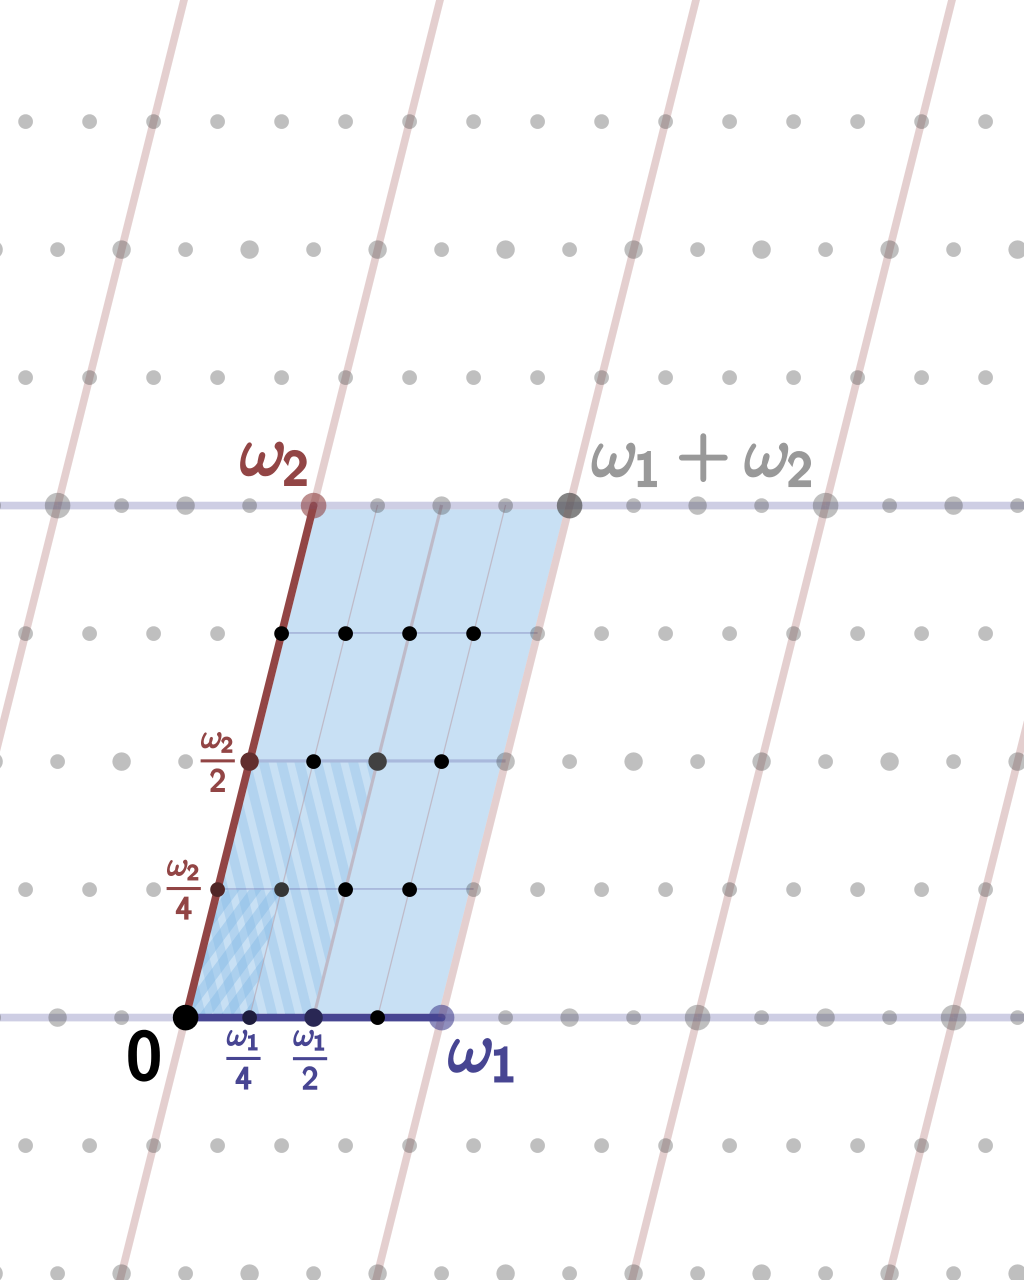
\includegraphics[width=0.7\textheight]{images/lattice.png}
	\end{figure}\fn{\tiny S. Derbyshire, \emph{Lattice torsion points}. CC BY-SA 3.0}
\end{frame}




% Lattice 2
\begin{frame}[plain]
	\begin{figure}[!ht]
	\centering
	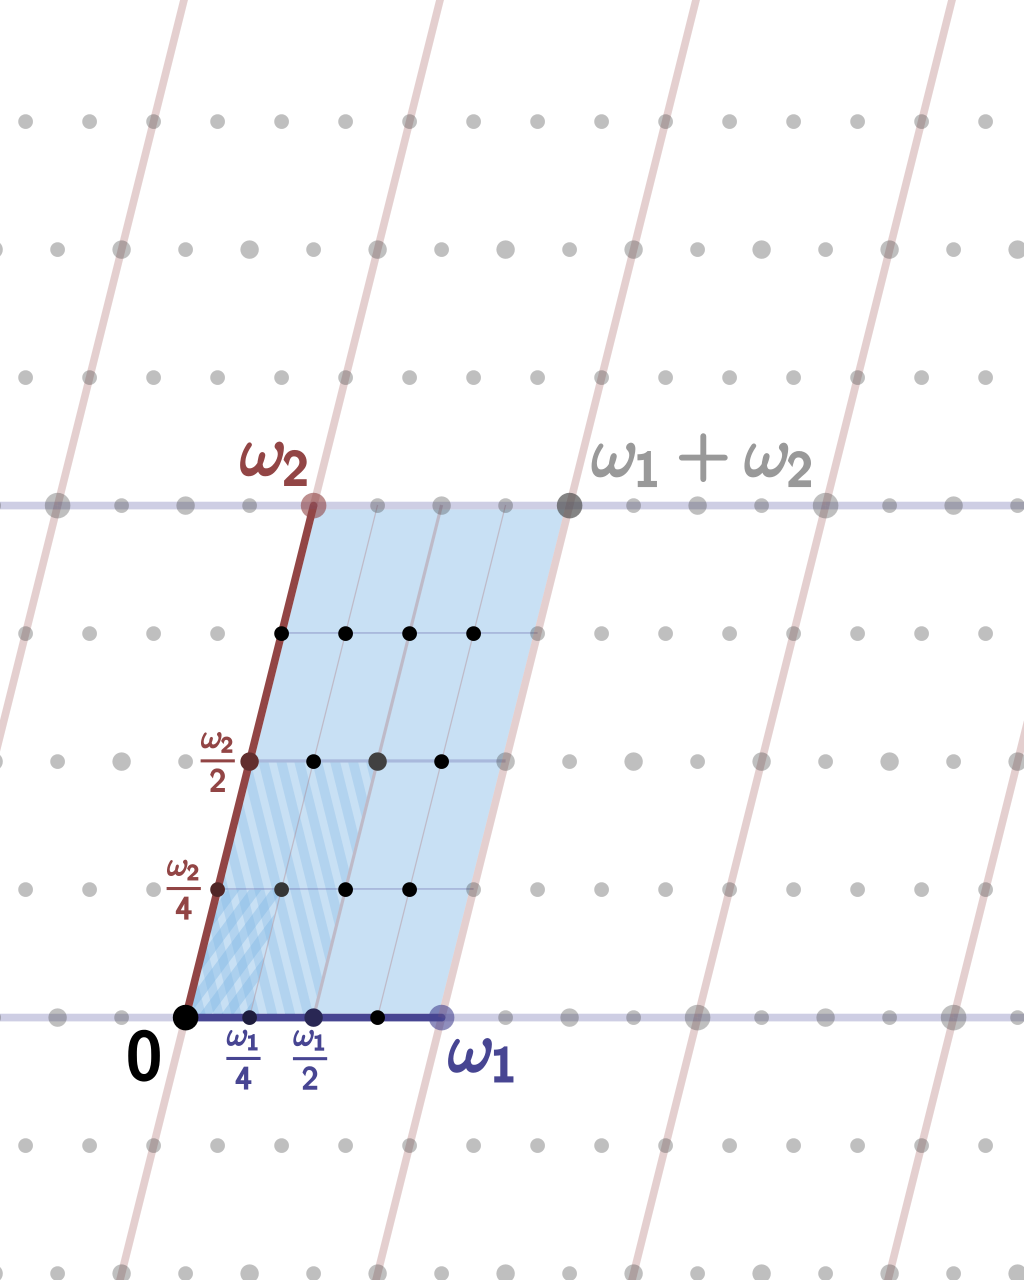
\includegraphics[width=0.3\textwidth]{images/lattice.png}
	\end{figure}

\begin{itemize}
\item This shows: $E[n]:= \{ P \in E \colon nP= \O \} \cong \Z/n\Z \oplus \Z/n\Z$
\item $E(\C)$ is isomorphic to a torus
	\begin{figure}[!ht]
	\centering
	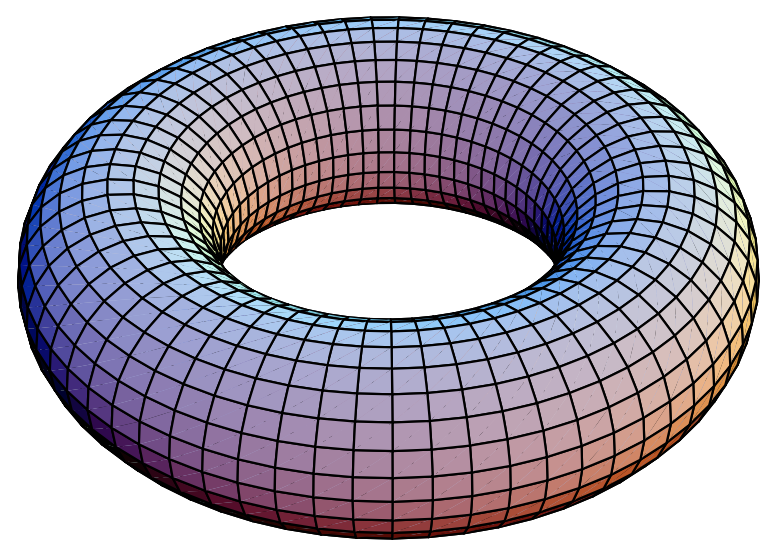
\includegraphics[width=0.3\textwidth]{images/torus.png}
	\end{figure}
\end{itemize}
\end{frame}




% E(K) Torsion Structure
\begin{frame}[plain]
\frametitle{\textcolor{white}{Structure of the Torsion Subgroup}}
	\[
	\begin{split}
	E(K)_{\text{tors}} &\cong\; \qfrac{\Z}{m\Z} \oplus \qfrac{\Z}{mn\Z} \\[0.5cm]
	E[n] &\cong\; \qfrac{\Z}{n\Z} \oplus \qfrac{\Z}{n\Z}
	\end{split}
	\]
\end{frame}



% Galois Representation
\begin{frame}[plain]
\frametitle{\textcolor{white}{Galois Representations}}

\begin{itemize}
\item Let $G_K:= \Gal(\overline{K}/K)$ be the absolute Galois group of $K$. 

\item $G_K$ acts on $E[n] \cong \Z/n\Z \oplus \Z/n\Z$

\item Fix a basis of $\Z/n\Z \oplus \Z/n\Z$, then we have a representation
	\[
	\rho_{E,n}: G_K \to \Aut(E[n]) \simeq \GL_2(\Z/n\Z),
	\]
the so-called mod $n$ Galois representation. 

\item One also forms the $\ell$-adic Tate module: $T_\ell(E):= \varprojlim_n E[\ell^n]$ and the $\ell$-adic representation $\rho_\ell: G_K \to \Aut(T_\ell(E))$. 
\end{itemize}

\begin{thm}[Serre]
Let $K$ be a number field, and let $E/K$ be an elliptic curve without CM. Then for all but finitely many primes $\ell$, $\rho_{E,\ell}: G_K \to \GL_2(\F_\ell)$ is surjective. 
\end{thm}
\end{frame}



% L-functions
\begin{frame}[plain]
\frametitle{\textcolor{white}{$L$-functions}}

Hasse Principle: $|p+1- \#E(\F_p)| \leq 2 \sqrt{p}$. We define `error terms' $a_p:= p + 1 - \#E(\F_p)$.  \par \vspace{0.5cm}

Then we define the Hasse-Weil $L$-function of $E$ to be
	\[
	L(E,s)= \prod_{p \nmid \Delta} \dfrac{1}{1 - a_p p^{-s} + p^{1-2s}}
	\] 
We can also write
	\[
	L(E,s)= \sum_{n \geq 1} \dfrac{a_n}{n^s},
	\]
where $a_n$ are the Fourier coefficients given by
	\[
	a_p=
	\begin{cases}
	p+1-N_p, & \text{if } E \text{ has good reduction at } p \\
	1, & \text{if } E \text{ has split multiplicative reduction at } p \\
	-1, & \text{if } E \text{ has non-split multiplicative reduction at } p \\
	0, & \text{if } E \text{ has additive reduction at } p
	\end{cases}
	\]
\end{frame}



% Modularity Theorem
\begin{frame}[plain]
\begin{thm}[Wiles, Taylor, Brueil, Conrad, Diamond]
$L(E,s)$ can be analytically continued to $\C$.
\end{thm}
	\begin{figure}[h]
	\centering
	\begin{subfigure}{0.3\textwidth}
	\captionsetup{labelformat=empty}
	\centering
	\fbox{
\includegraphics[width=0.6\textwidth]{images/wiles.jpg}}
	\caption{\scriptsize Andrew Wiles}
	\end{subfigure}
	%
	\begin{subfigure}{0.3\textwidth}
	\captionsetup{labelformat=empty}
	\centering
	\fbox{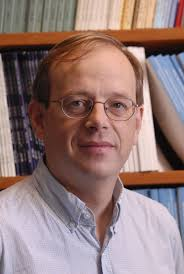
\includegraphics[width=0.43\textwidth]{images/taylor.jpeg}}
	\caption{\scriptsize Richard Taylor}
	\end{subfigure}
	%
	\begin{subfigure}{0.3\textwidth}
	\captionsetup{labelformat=empty}
	\centering
	\fbox{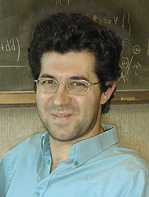
\includegraphics[width=0.5\textwidth]{images/breuil.jpg}}
	\caption{\scriptsize Christophe Breuil}
	\end{subfigure}
	%
	\\
	\begin{subfigure}{0.4\textwidth}
	\captionsetup{labelformat=empty}
	\centering
	\fbox{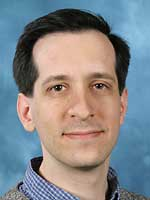
\includegraphics[width=0.35\textwidth]{images/conrad.jpg}}
	\caption{\scriptsize Brian Conrad}
	\end{subfigure}
	%
	\begin{subfigure}{0.4\textwidth}
	\captionsetup{labelformat=empty}
	\centering
	\fbox{
\includegraphics[width=0.35\textwidth]{images/diamond.jpg}}
	\caption{\scriptsize Fred Diamond}
	\end{subfigure}
	\end{figure}
\end{frame}



% Taylor Expansion
\begin{frame}[plain]
In particular, $L(E,s)$ has a Taylor expansion about $s=1$: \vspace{0.3cm}

	\[
	L(E,s)= c_0 + c_1 (s-1) + c_2(s-1)^2 + \cdots
	\]  \vspace{0.3cm}
	
Define the analytic rank $r_{an}$ of $E$ to be the order of vanishing of $L(E,s)$ at $s=1$, \vspace{0.3cm}

	\[
	L(E,s)= c_{r_{an}} (s - 1)^{r_{an}} + \cdots
	\] 
\end{frame}



% BSD
\begin{frame}[plain]

\begin{conj}[BSD]
The algebraic and analytic ranks of elliptic curves are equal.
\end{conj} 
	\begin{figure}[h]
	\centering
	\begin{subfigure}{0.3\textwidth}
	\captionsetup{labelformat=empty}
	\centering
	\fbox{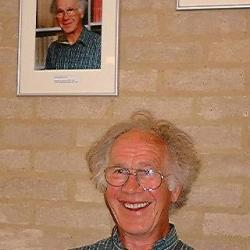
\includegraphics[width=0.7\textwidth]{images/birch.jpg}}
	\caption{Bryan Birch \\ \phantom{x}}
	\end{subfigure}
	%
	\begin{subfigure}{0.6\textwidth}
	\captionsetup{labelformat=empty}
	\centering
	\fbox{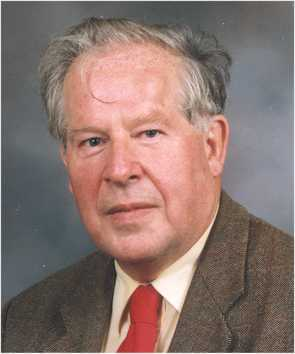
\includegraphics[width=0.3\textwidth]{images/dyer.jpg}}
	\caption{(Sir Henry) Peter \\ Francis Swinnerton-Dyer}
	\end{subfigure}
	\end{figure} \vspace{0.3cm}

Due to work of Gross, Zagier, Kolyvagin, if $r_{an} \leq 1$, then $r_{\text{anal}}=r_{alg}$.
If BSD is true, there is an algorithm to compute the rank of an elliptic curve. 

	\[
	\lim_{s \to 1} \dfrac{L(E,s)}{(s-1)^{r_E}} = \dfrac{\Omega_E \, \Reg(E) \, \#\sha(E/\Q) \, \prod_p c_p}{\#E(\Q)_{tors}^2}
	\]
\end{frame}



% Boundedness
\begin{frame}[plain]
\ctext{Boundedness}
\end{frame}



% Bounded 2
\begin{frame}[plain] \frametitle{Boundedness of Torsion} \footnotesize
One should ask why there should be finitely many possible torsion subgroups at all. The boundedness of the size of the torsion subgroup is a result of several individuals, originating with Merel in 1996. 

\begin{thm}[Merel,1996]
Let $K$ be a number field of degree $[K:\Q]=d>1$. There is a number $B(d)>0$ such that $|E(K)_\tors| \leq B(d)$ for all elliptic curves $E/K$.
\end{thm}
	\begin{figure}
	\captionsetup{labelformat=empty}
	\centering
	\fbox{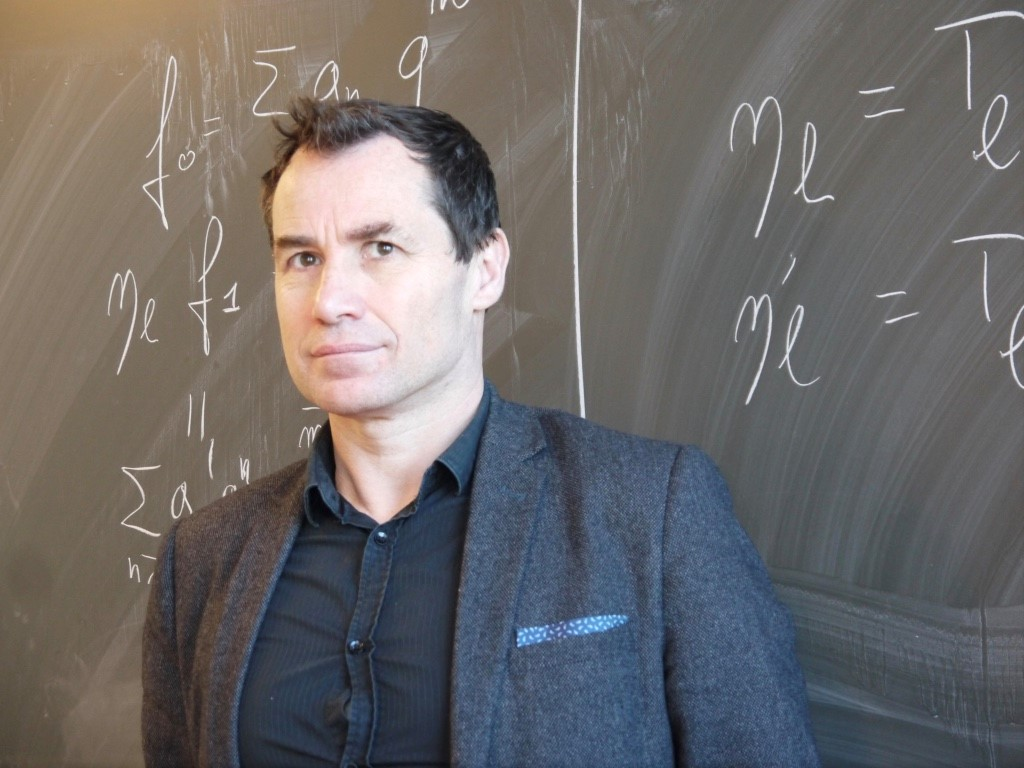
\includegraphics[width=0.50\textwidth]{images/merel.jpg}}
	\caption{Lo\"ic Merel}
	\end{figure}
\end{frame}



% Boundedness: Merel, Parent
\begin{frame}[plain] \scriptsize
\begin{thm}[Merel, 1996; Parent, 1999]
Let $K$ be a number field of degree $d > 1$. Then
	\begin{enumerate}[(i)]
	\item (Merel) Let $E/K$ be an elliptic curve. If $E(K)$ contains a point of exact prime order $p$, then $\ell \leq d^{3d^2}$.
	\item (Parent) If $P$ is a point of exact prime power order $\ell^n$, then
		\begin{enumerate}[(a)] \scriptsize
		\item $\ell^n \leq 65(3^d - 1)(2d)^6$, if $\ell \geq 5$
		\item $\ell^n \leq 65(5^d - 1)(2d)^6$, if $\ell= 3$
		\item $\ell^n \leq 129(3^d - 1)(3d)^6$, if $\ell= 2$
		\end{enumerate}
	In particular, $\ell^p \leq 129(5^d - 1)(3d)^6$ for all primes $\ell$. 
	\item (Oesterl\'e) If $p \in S(d)$, then $p \leq (1 + 3^{d/2})^2$. 
	\end{enumerate}
\end{thm}
	\begin{figure}[h]
	\centering
	\begin{subfigure}{0.3\textwidth}
	\captionsetup{labelformat=empty}
	\centering
	\fbox{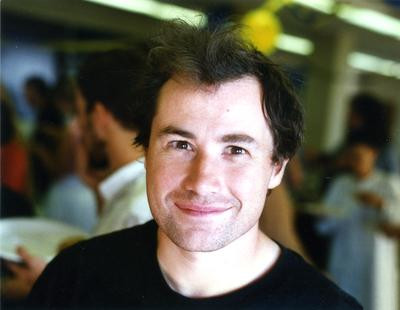
\includegraphics[width=0.92\textwidth]{images/merel.jpeg}}
	\caption{Lo\"ic Merel}
	\end{subfigure}
	%
	\begin{subfigure}{0.3\textwidth}
	\captionsetup{labelformat=empty}
	\centering
	\fbox{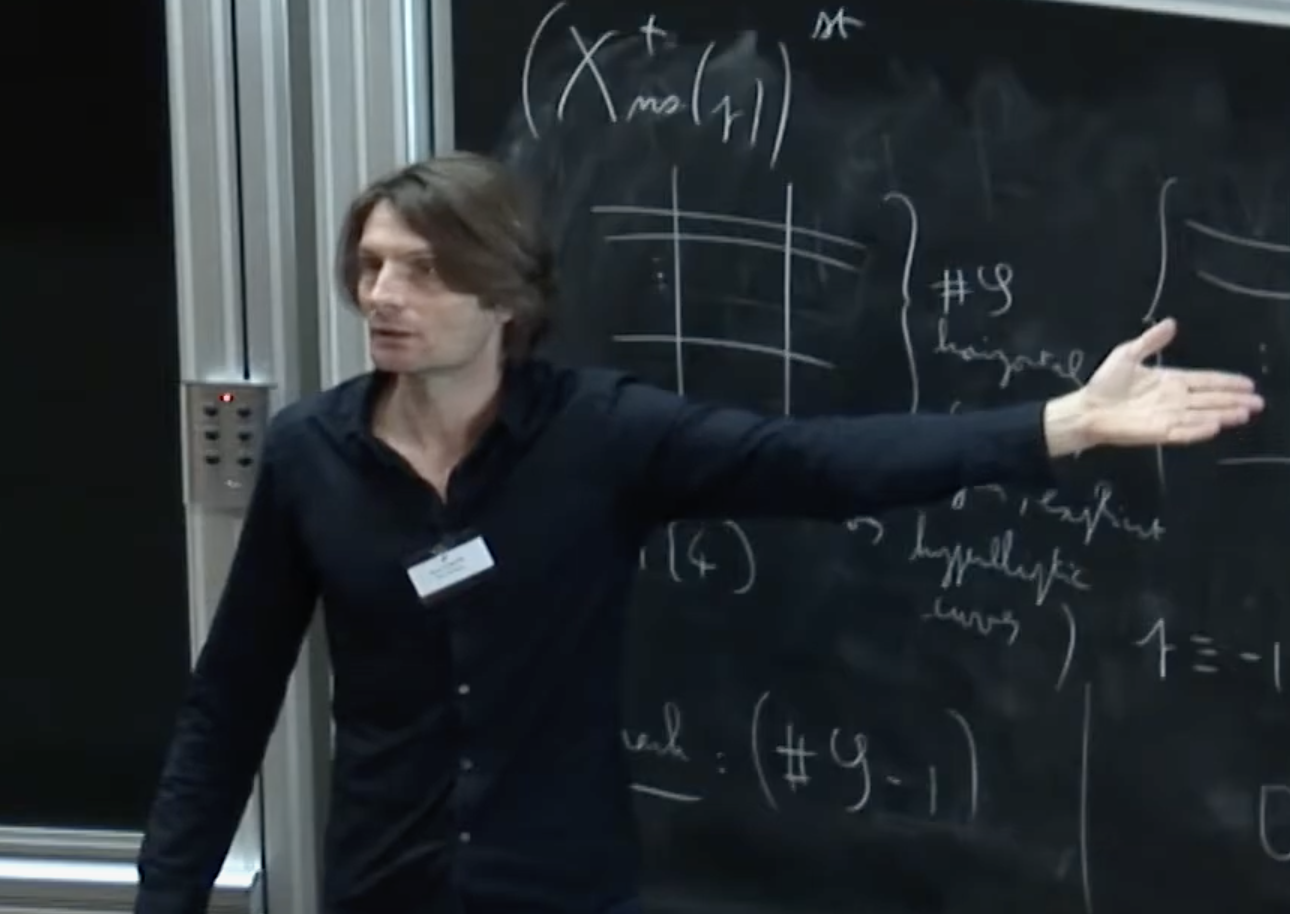
\includegraphics[width=\textwidth]{images/parent.png}}
	\caption{Pierre Parent}
	\end{subfigure} \hspace{0.05cm}
	%
	\begin{subfigure}{0.3\textwidth}
	\captionsetup{labelformat=empty}
	\centering
	\fbox{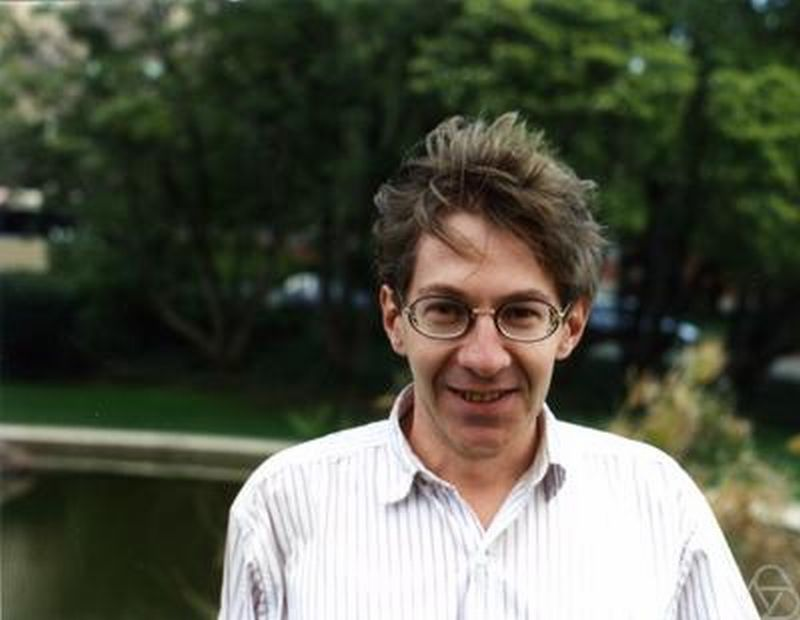
\includegraphics[width=0.92\textwidth]{images/oesterle.jpeg}}
	\caption{Joseph Oesterl\'e}
	\end{subfigure}
	\end{figure}
\end{frame}



% Conj
\begin{frame}[plain]
\begin{conj}[Clark, Cook, Stakewicz]
There is a constant $C$ such that $B(d) \leq C\, d \log\log d$ for all $d \geq 3$.
\end{conj}
	\begin{figure}[h]
	\centering
	\begin{subfigure}{0.3\textwidth}
	\captionsetup{labelformat=empty}
	\centering
	\fbox{
\includegraphics[width=0.70\textwidth]{images/clark.jpg}}
	\caption{Pete Clark}
	\end{subfigure} \quad
	%
	\begin{subfigure}{0.3\textwidth}
	\captionsetup{labelformat=empty}
	\centering
	\fbox{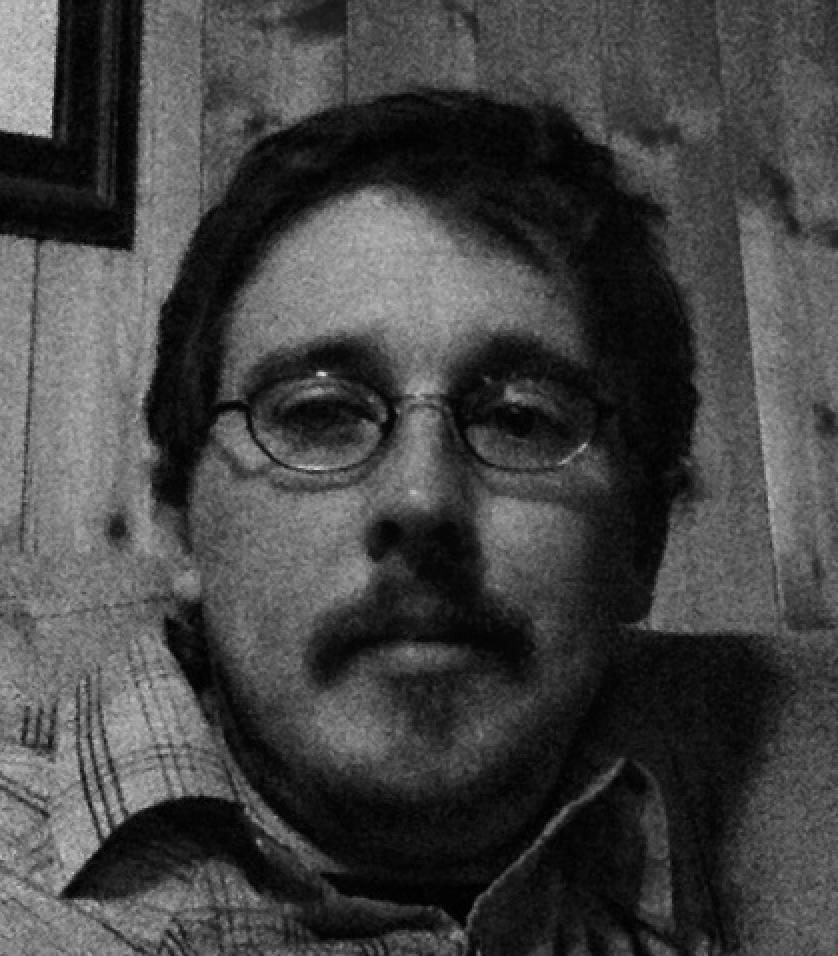
\includegraphics[width=0.82\textwidth]{images/cook.png}}
	\caption{Brian Cook}
	\end{subfigure}
	%
	\begin{subfigure}{0.3\textwidth}
	\captionsetup{labelformat=empty}
	\centering
	\fbox{
\includegraphics[width=0.65\textwidth]{images/stankewicz.png}}
	\caption{James Stankewicz}
	\end{subfigure}
	\end{figure}
\end{frame}


% Silverman
\begin{frame}[plain]
\begin{thm}[Hindry, Silverman, 1999]
Let $K$ be a field of degree $d \geq 2$ and $E/K$ be an elliptic curve such that $j(E)$ is an algebraic integer. Then we have
	\[
	|E(K)_\tors| \leq 1\,977\,404 \cdot d \log d
	\]
\end{thm}
	\begin{figure}[h]
	\centering
	\begin{subfigure}{0.3\textwidth}
	\captionsetup{labelformat=empty}
	\centering
	\fbox{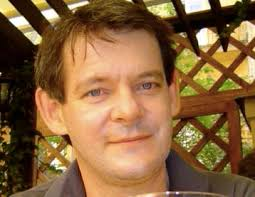
\includegraphics[width=1.0\textwidth]{images/hindry.jpeg}}
	\caption{Marc Hindry}
	\end{subfigure}
	%
	\begin{subfigure}{0.3\textwidth}
	\captionsetup{labelformat=empty}
	\centering
	\fbox{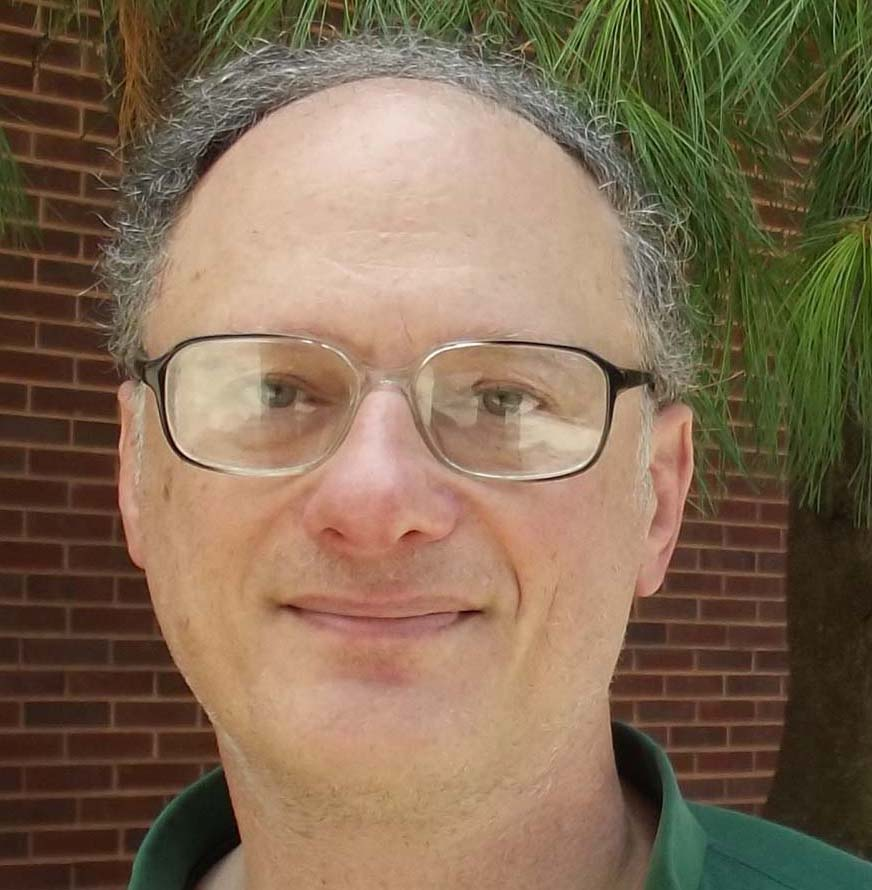
\includegraphics[width=0.77\textwidth]{images/silverman.jpg}}
	\caption{Joseph Silverman}
	\end{subfigure}
	\end{figure}
\end{frame}


% Clark, Pollack
\begin{frame}[plain]
\begin{thm}[Clark, Pollack, 2015]
There is an absolute, effective constant $C$ such that for all number fields $K$ of degree $d \geq 3$ and all elliptic curves $E/K$ with CM, we have $|E(K)_\tors| \leq C\, d \log \log d$.
\end{thm}
	\begin{figure}[h]
	\centering
	\begin{subfigure}{0.3\textwidth}
	\captionsetup{labelformat=empty}
	\centering
	\fbox{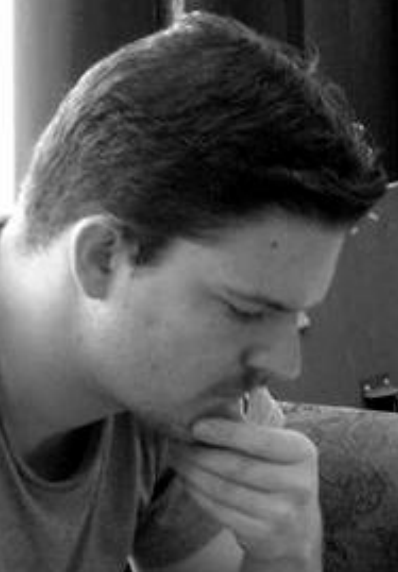
\includegraphics[width=0.62\textwidth]{images/clark2.png}}
	\caption{Pete Clark}
	\end{subfigure}
	%
	\begin{subfigure}{0.3\textwidth}
	\captionsetup{labelformat=empty}
	\centering
	\fbox{
\includegraphics[width=0.90\textwidth]{images/pollack.jpg}}
	\caption{Paul Pollack}
	\end{subfigure}
	\end{figure}
\end{frame}


% Prime Point
\begin{frame}[plain]
\begin{thm}[Merel, 1996]
Let $F/\Q$ be a number field of degree $d$. If $P \in E(F)$ is a point of exact prime power $p^n$, then $p \leq 3^{3d^2}$.
\end{thm} 
	\begin{figure}[h]
	\centering
	\begin{subfigure}{0.3\textwidth}
	\captionsetup{labelformat=empty}
	\centering
	\fbox{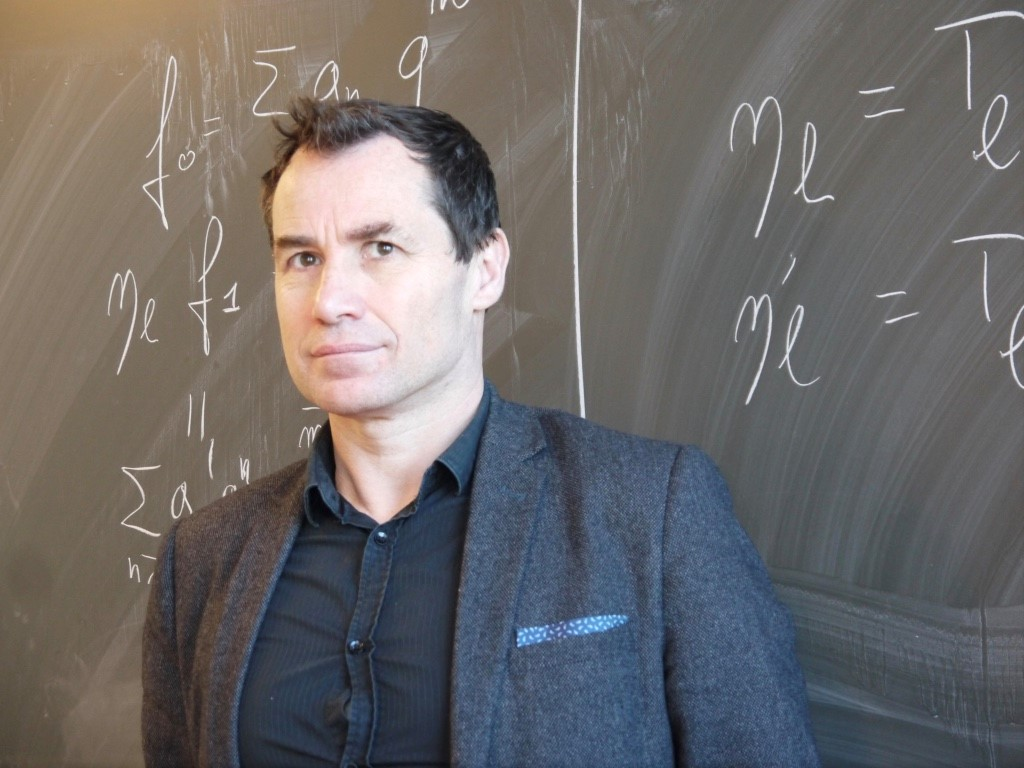
\includegraphics[width=0.90\textwidth]{images/merel.jpg}}
	\caption{Lo\"ic Merel}
	\end{subfigure}
	%
	\begin{subfigure}{0.3\textwidth}
	\captionsetup{labelformat=empty}
	\centering
	\fbox{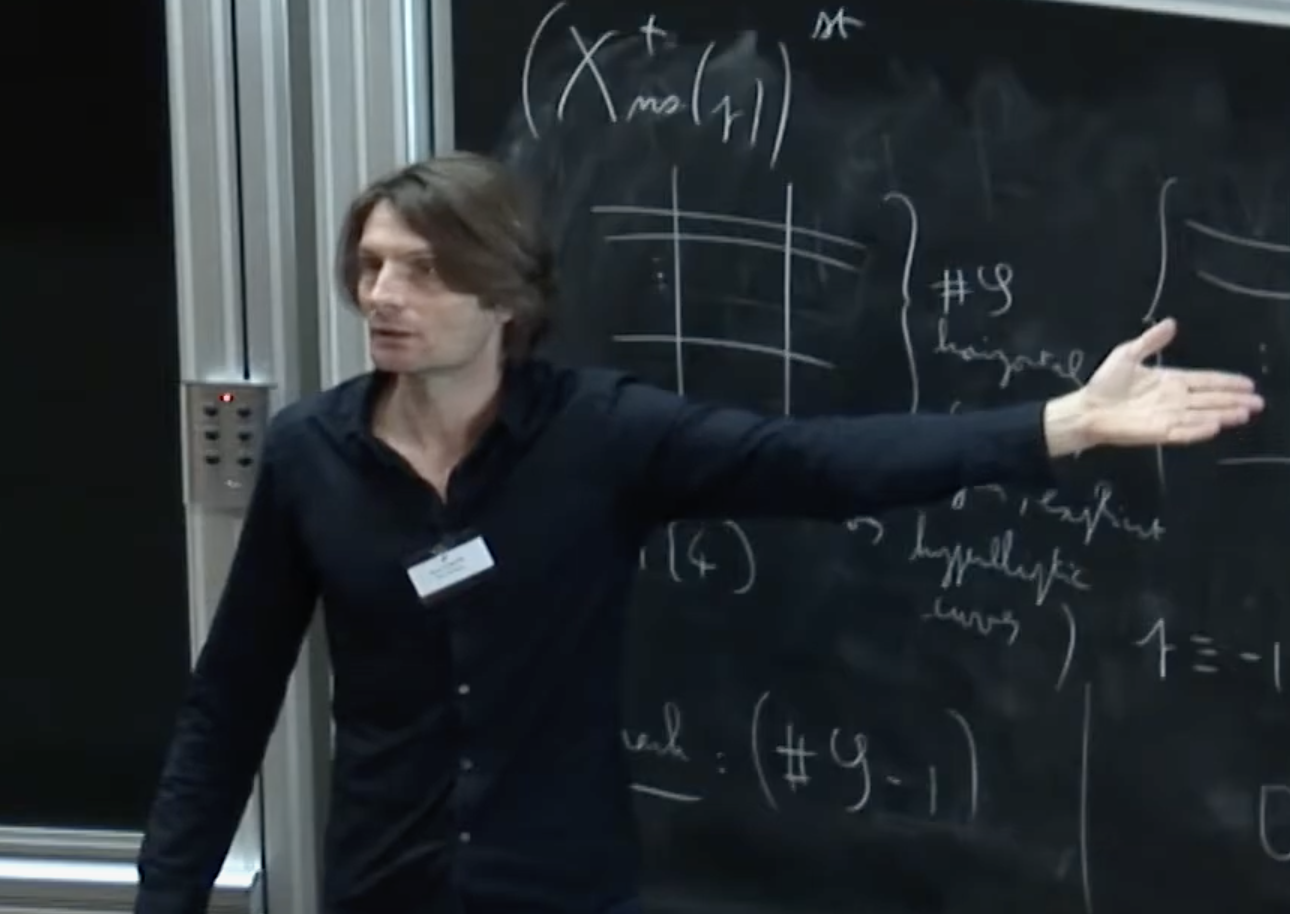
\includegraphics[width=0.95\textwidth]{images/parent.png}}
	\caption{Pierre Parent}
	\end{subfigure}
	\end{figure}
\begin{rem}
In 1999, Parent improved this to $p^n \leq 129(5^d - 1)(3d)^6$.
\end{rem}
\end{frame}


% Lozano Prime
\begin{frame}[plain]
\begin{thm}[Lozano-Robledo, 2013]
Let $K/\Q$ be a number field of degree $d$ and suppose there is an elliptic curve $E/K$ with CM by a full order with a point of order $p^n$, then
	\[
	\varphi(p^n) \leq 24\, e_{\max}(p,K/\Q) \leq 24\, d
	\]
\end{thm}
	\begin{figure}[h]
	\centering
	\begin{subfigure}{\textwidth}
	\captionsetup{labelformat=empty}
	\centering
	\fbox{
\includegraphics[width=0.25\textwidth]{images/robledo.jpg}}
	\caption{\'Alvaro Lozano-Robledo}
	\end{subfigure}
	\end{figure}
\end{frame}



% Torsion Results
\begin{frame}[plain]
\ctext{Torsion over General Number Fields}
\end{frame}



% Quadratic Number Field
\begin{frame}[plain]
\begin{thm}[Kenku, Momose, 1988; Kamienny, 1992]
 Let $K/\Q$ be a quadratic number field and $E/K$ be an elliptic curve. Then the possible torsion subgroups $E(K)_\tors$ are precisely:
 	\[
	\begin{cases}
	\Z/n\Z, & \text{with } n=1,2,\ldots,16,18 \text{ or} \\
	\Z/2\Z \oplus \Z/2n\Z, & \text{with } n=1,\ldots,6 \text{ or} \\
	\Z/3\Z \oplus \Z/3n\Z, & \text{with } n=1,2 \text{ or} \\
	\Z/4\Z \oplus \Z/4\Z
	\end{cases}
	\]
Moreover, each possibility occurs infinitely often. 
\end{thm}
	\begin{figure}[h]
	\centering
	\begin{subfigure}{0.3\textwidth}
	\captionsetup{labelformat=empty}
	\centering
	\fbox{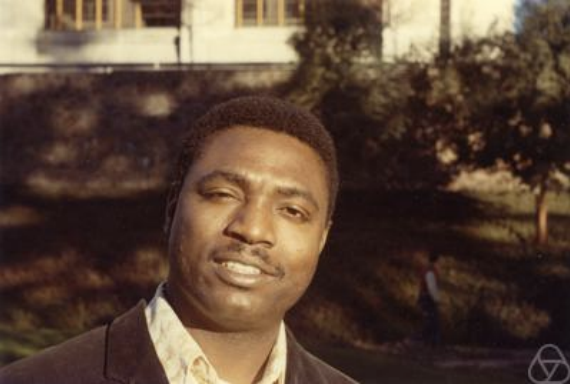
\includegraphics[width=0.9\textwidth]{images/kenku.png}}
	\caption{Monsur Kenku}
	\end{subfigure} \;\;\;
	%
	\begin{subfigure}{0.3\textwidth}
	\captionsetup{labelformat=empty}
	\centering
	\fbox{
\includegraphics[width=0.85\textwidth]{images/momose.png}}
	\caption{Fumiyuki Momose}
	\end{subfigure}
	%
	\begin{subfigure}{0.3\textwidth}
	\captionsetup{labelformat=empty}
	\centering
	\fbox{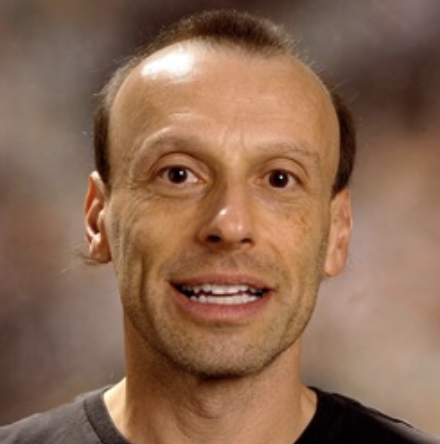
\includegraphics[width=0.63\textwidth]{images/kamienny.png}}
	\caption{Sheldon Kamienny}
	\end{subfigure}
	\end{figure}
\end{frame}



% Cubic Number Field
\begin{frame}[plain,c]
\footnotesize
\begin{thm}[Jeon,Kim,Schweizer, 2004; Etropolski,Morrow,Zureick Brown; Derickx, 2016; Derickx,Etropolski,van Hoeij,Morrow,Zureick-Brown, 2020]
Let $K/\Q$ be a cubic number field and $E/K$ be an elliptic curve. Then the possible torsion subgroups $E(K)_\tors$ are precisely:
	\[
	\begin{cases}
	\Z/n\Z, & \text{with } n=1,2,\ldots,16,18,20,21 \text{ or} \\
	\Z/2n\Z, & \text{with }n=1,\ldots,7
	\end{cases}
	\] 
Each of these possibilities occurs infinitely many times except for $\Z/21\Z$ which occurs only for the elliptic curve \texttt{162b1} over $\Q(\zeta_9)^+$.
\end{thm}
	\begin{figure}[h]
	\centering
	\begin{subfigure}{0.10\textwidth}
	\captionsetup{labelformat=empty}
	\centering
	\fbox{
\includegraphics[width=1.2\textwidth]{images/jeon.png}}
	\caption{\hspace{0.2cm}\scriptsize{Jeon}}
	\end{subfigure} \quad\quad
	%
	\begin{subfigure}{0.10\textwidth}
	\captionsetup{labelformat=empty}
	\centering
	\fbox{
\includegraphics[width=1.2\textwidth]{images/kim.jpg}}
	\caption{\hspace{0.3cm}\scriptsize{Kim}}
	\end{subfigure} \quad\quad
	%
	\begin{subfigure}{0.10\textwidth}
	\captionsetup{labelformat=empty}
	\centering
	\fbox{
\includegraphics[width=1.2\textwidth]{images/schweizer.jpeg}}
	\caption{\hspace{0.1cm}\scriptsize{Schweizer}}
	\end{subfigure} \\
	%
	\hfill
	\begin{subfigure}{0.12\textwidth}
	\captionsetup{labelformat=empty}
	\centering
	\fbox{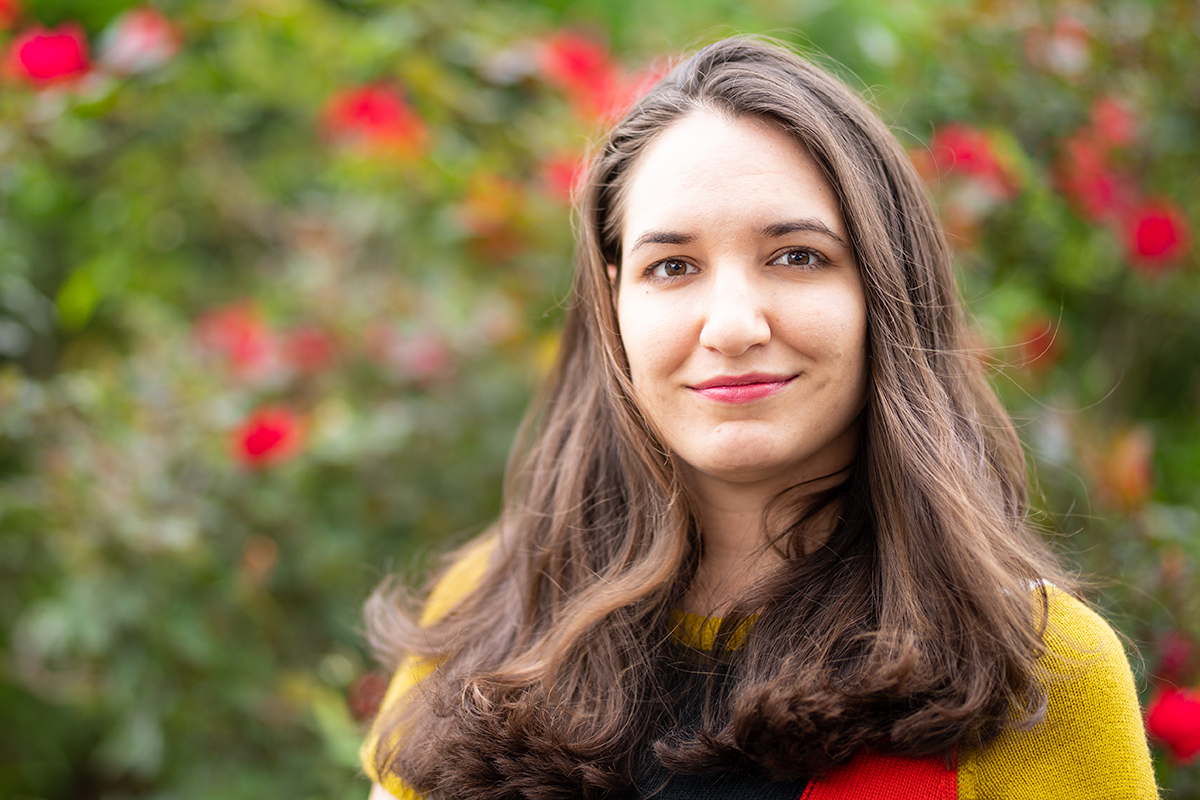
\includegraphics[width=1.7\textwidth]{images/etropolski.jpg}}
	\caption{\;\;\;\;\scriptsize{Etropolski}}
	\end{subfigure} \hspace{1.5cm}
	%
	\begin{subfigure}{0.10\textwidth}
	\captionsetup{labelformat=empty}
	\centering
	\fbox{
\includegraphics[width=1.45\textwidth]{images/morrow.png}}
	\caption{\;\;\;\scriptsize{Morrow}}
	\end{subfigure} \hspace{0.6cm}
	%
	\begin{subfigure}{0.192\textwidth}
	\captionsetup{labelformat=empty}
	\centering
	\fbox{
\includegraphics[width=0.55\textwidth]{images/zbrown3.jpeg}}
	\caption{\scriptsize Zureick-Brown}
	\end{subfigure} \hspace{0cm}
	%
	\begin{subfigure}{0.09\textwidth}
	\captionsetup{labelformat=empty}
	\centering
	\fbox{
\includegraphics[width=1.2\textwidth]{images/derickx.jpg}}
	\caption{\;\;\scriptsize{Derickx}}
	\end{subfigure} \hfill \phantom{.}
	\begin{subfigure}{0.115\textwidth}
	\captionsetup{labelformat=empty}
	\centering
	\fbox{
\includegraphics[width=1.2\textwidth]{images/hoeij.jpeg}}
	\caption{\;\;\tiny{van Hoeij}}
	\end{subfigure} \hfill \phantom{.}
	\end{figure}
\end{frame}





% Quartic Number Field
\begin{frame}[plain]
\begin{thm}[Jeon, Kim, Park, 2006]
Let $K/\Q$ be a quartic number field and $E/K$ be an elliptic curve. Then the possible torsion subgroups $E(K)_\tors$ appearing infinitely often are precisely:
	\[
	\begin{cases}
	\Z/n\Z, & \text{with } n=1,2,\ldots,18,20,21,22 \text{ or} \\
	\Z/2\Z \oplus \Z/2n\Z, & \text{with } n=1,\ldots,9 \text{ or} \\
	\Z/3\Z \oplus \Z/3n\Z, & \text{with } n=1,2,3 \text{ or} \\
	\Z/4\Z \oplus \Z/4n\Z, & \text{with } n=1,2 \text{ or} \\
	\Z/5\Z \oplus \Z/5\Z & \text{ or} \\
	\Z/6\Z \oplus \Z/6\Z
	\end{cases}
	\]
\end{thm}
	\begin{figure}[h]
	\centering
	\begin{subfigure}{0.3\textwidth}
	\captionsetup{labelformat=empty}
	\centering
	\fbox{
\includegraphics[width=0.60\textwidth]{images/jeon.png}}
	\caption{\hspace{0.1cm}Daeyeol Jeon}
	\end{subfigure}
	%
	\begin{subfigure}{0.3\textwidth}
	\captionsetup{labelformat=empty}
	\centering
	\fbox{
\includegraphics[width=0.63\textwidth]{images/kim.jpg}}
	\caption{Chang Kim}
	\end{subfigure}
	%
	\begin{subfigure}{0.3\textwidth}
	\captionsetup{labelformat=empty}
	\centering
	\fbox{
\includegraphics[width=0.45\textwidth]{images/park.png}}
	\caption{\hspace{0cm}Eui-Sung Park}
	\end{subfigure}
	\end{figure}
\end{frame}



% Quintic Number Field
\begin{frame}[plain]
\begin{thm}[Derickx, Sutherland, 2016]
Let $K/\Q$ be a quintic number field and $E/K$ be an elliptic curve. Then the possible torsion subgroups $E(K)_\tors$ appearing infinitely often are precisely:
	\[
	\begin{cases}
	\Z/n\Z, & \text{with } n=1,\ldots,22,24,25 \text{ or} \\
	\Z/2\Z \oplus \Z/2n\Z, & \text{with } n=1,\ldots,8
	\end{cases}
	\]
\end{thm}
	\begin{figure}[h]
	\centering
	\begin{subfigure}{0.3\textwidth}
	\captionsetup{labelformat=empty}
	\centering
	\fbox{
\includegraphics[width=0.72\textwidth]{images/derickx.jpg}}
	\caption{\hspace{0.1cm}Maarten Derickx}
	\end{subfigure}
	%
	\begin{subfigure}{0.3\textwidth}
	\captionsetup{labelformat=empty}
	\centering
	\fbox{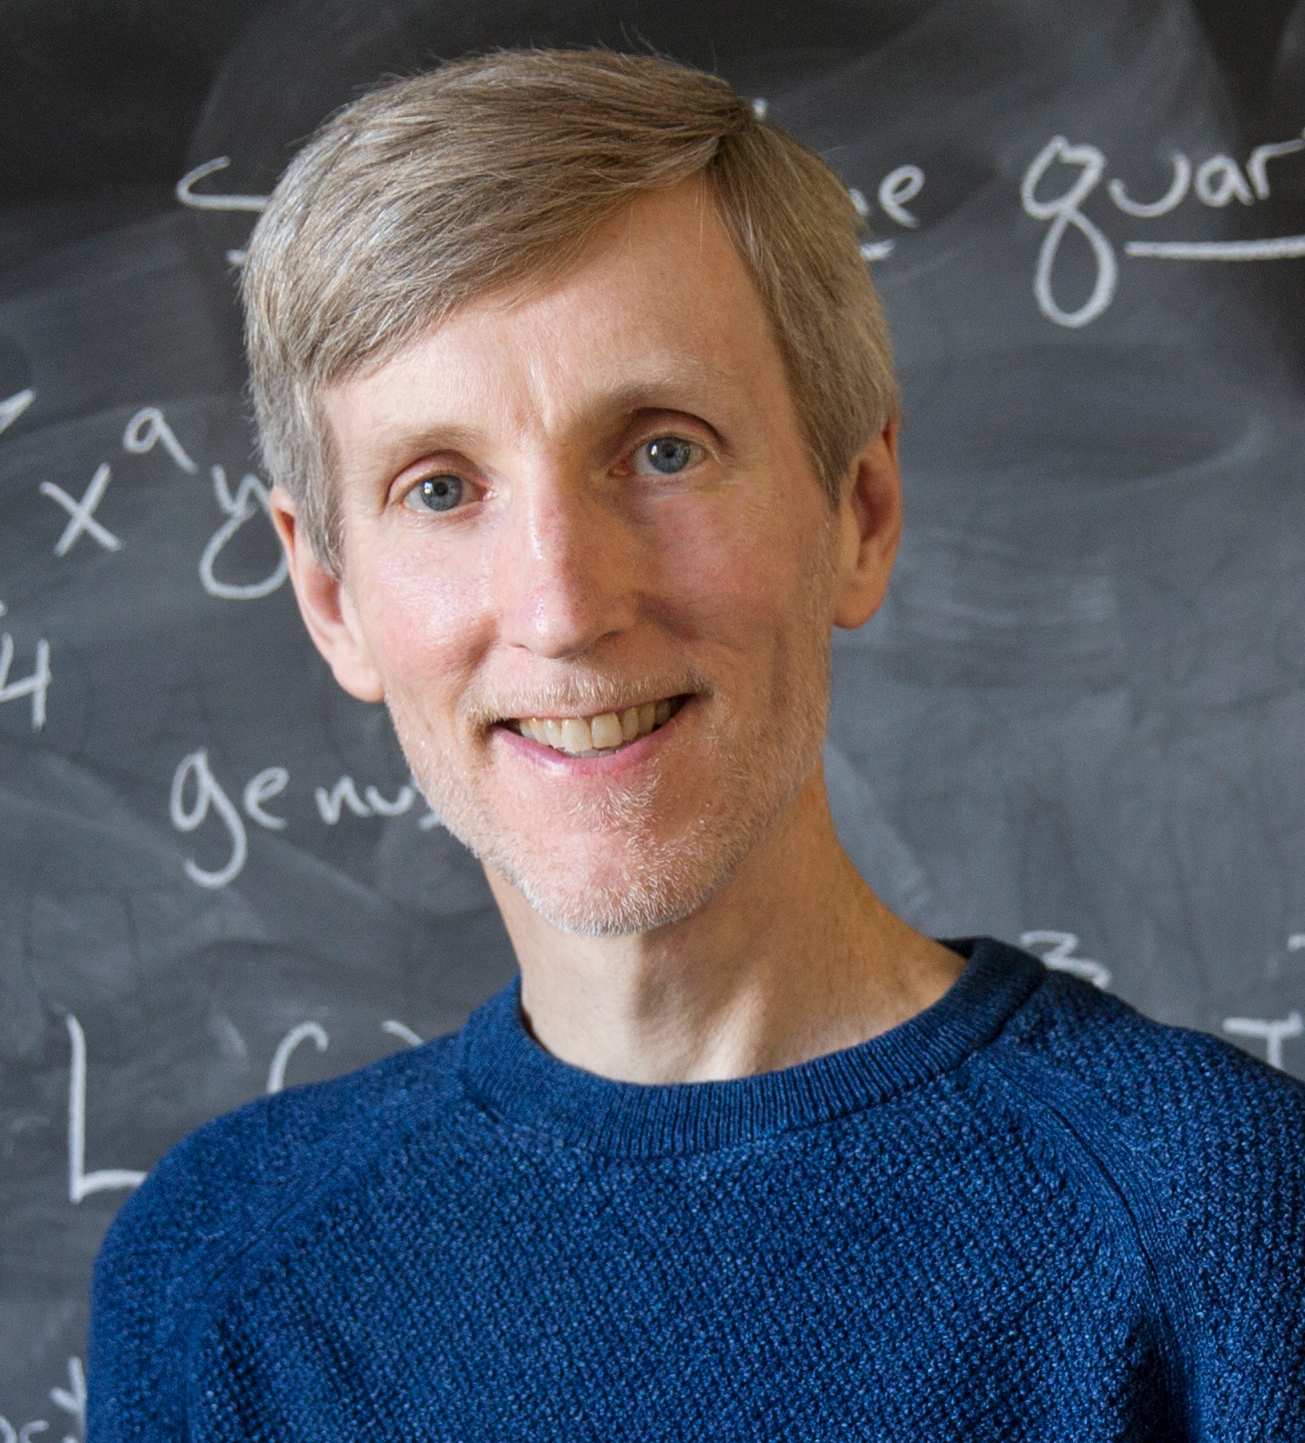
\includegraphics[width=0.82\textwidth]{images/sutherland.jpg}}
	\caption{Drew Sutherland}
	\end{subfigure}
	\end{figure}
\end{frame}



% Sextic Number Field
\begin{frame}[plain]
\begin{thm}[Derickx, Sutherland, 2016]
Let $K/\Q$ be a sextic number field and $E/K$ be an elliptic curve. Then the possible torsion subgroups $E(K)_\tors$ appearing infinitely often are precisely:
	\[
	\begin{cases}
	\Z/n\Z, &  \text{with } n=1,\ldots,30; n \neq 23,25,29 \text{ or} \\
	\Z/2\Z \oplus \Z/2n\Z, & \text{with } n=1,\ldots,10 \text{ or} \\
	\Z/3\Z \oplus \Z/3n\Z, & \text{with } n=1,\ldots,4 \text{ or} \\
	\Z/4\Z \oplus \Z/4n\Z, & \text{with } n=1,2 \text{ or} \\
	\Z/6\Z \oplus \Z/6\Z 
	\end{cases}
	\]
\end{thm}
	\begin{figure}[h]
	\centering
	\begin{subfigure}{0.28\textwidth}
	\captionsetup{labelformat=empty}
	\centering
	\fbox{
\includegraphics[width=0.72\textwidth]{images/derickx.jpg}}
	\caption{\hspace{0.1cm}Maarten Derickx}
	\end{subfigure}
	%
	\begin{subfigure}{0.28\textwidth}
	\captionsetup{labelformat=empty}
	\centering
	\fbox{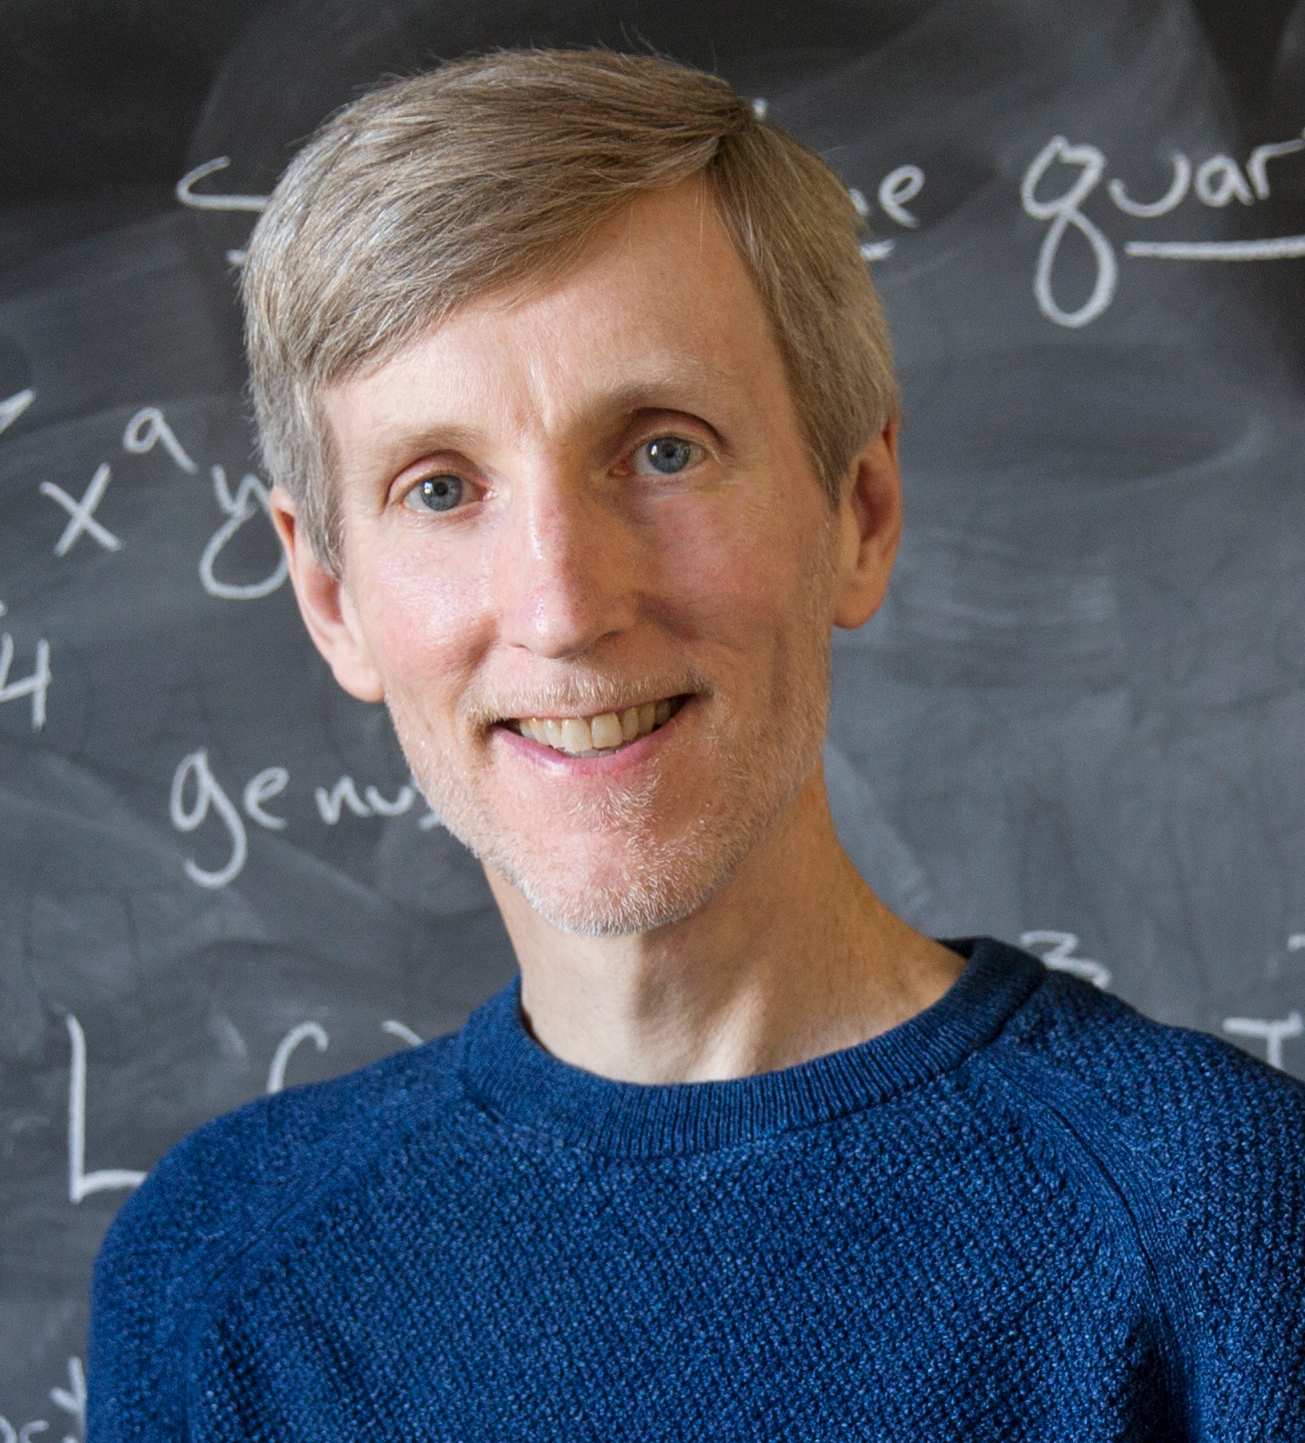
\includegraphics[width=0.82\textwidth]{images/sutherland.jpg}}
	\caption{Drew Sutherland}
	\end{subfigure}
	\end{figure}
\end{frame}





% CM Clark, Corn, Rice, Stankewicz
\begin{frame}[plain,c]
	\begin{thm}[Clark, Corn, Rice, Stankewicz; 2013]
	Let $K$ be a number field of degree $d=1,2,\ldots,13$ and $E/K$ be an elliptic curve with CM. Then all possible torsion subgroups are given, and an algorithm to compute the list.
	\end{thm} 
	\begin{figure}[h]
	\centering
	\begin{subfigure}{0.23\textwidth}
	\captionsetup{labelformat=empty}
	\centering
	\fbox{
\includegraphics[width=0.75\textwidth]{images/clark.jpg}}
	\caption{Pete Clark}
	\end{subfigure}
	%
	\begin{subfigure}{0.23\textwidth}
	\captionsetup{labelformat=empty}
	\centering
	\fbox{
\includegraphics[width=0.83\textwidth]{images/corn.jpg}}
	\caption{Patrick Corn}
	\end{subfigure}
	%
	\begin{subfigure}{0.23\textwidth}
	\captionsetup{labelformat=empty}
	\centering
	\fbox{
\includegraphics[width=1.0\textwidth]{images/rice.png}}
	\caption{Alex Rice}
	\end{subfigure}
	%
	\begin{subfigure}{0.25\textwidth}
	\captionsetup{labelformat=empty}
	\centering
	\fbox{
\includegraphics[width=0.65\textwidth]{images/stankewicz.png}}
	\caption{James Stankewicz}
	\end{subfigure}
	\end{figure}
\end{frame}




% CM Bourdon Clark Stankewicz
\begin{frame}[plain]
\footnotesize
\begin{thm}[Bourdon, Clark, Stankewicz, 2015]
Let $F$ be a number field of odd degree, let $E/F$ be a $K$-CM elliptic curve, and let $T= E(F)_\tors$. Then
	\begin{enumerate}[(a)]
	\item One of the following occurs:
		\begin{enumerate}[(i)] \footnotesize
		\item $T$ is isomorphic to the trivial group $\O$, $\Z/2\Z$, $\Z/4\Z$, or $\Z/2\Z \times \Z/2\Z$;
		\item $T \cong \Z/\ell^n\Z$ for a prime $\ell \equiv 3 \mod 8$ and $n \in \Z^+$ and $K= \Q(\sqrt{-\ell})$;
		\item $T \cong \Z/2\ell^n\Z$ for a prime $\ell \equiv 3 \mod 4$ and $n \in \Z^+$ and $K= \Q(\sqrt{-\ell})$. 
		\end{enumerate}
	\item If $E(F)_\tors \cong \Z/2\Z \oplus \Z/2\Z$, then $\End E$ has discriminant $\Delta= -4$.
	\item If $E(F)_\tors \cong \Z/4\Z$, then $\End E$ has discriminant $\Delta \in \{ -4, -16 \}$.
	\item Each of the groups listed in part (a) arises up to isomorphism as the torsion subgroup $E(F)$ of a CM elliptic curve $E$ defined over an odd degree number field $F$. 
	\end{enumerate}
\end{thm}
	\begin{figure}[h]
	\centering
	\begin{subfigure}{0.30\textwidth}
	\captionsetup{labelformat=empty}
	\centering
	\fbox{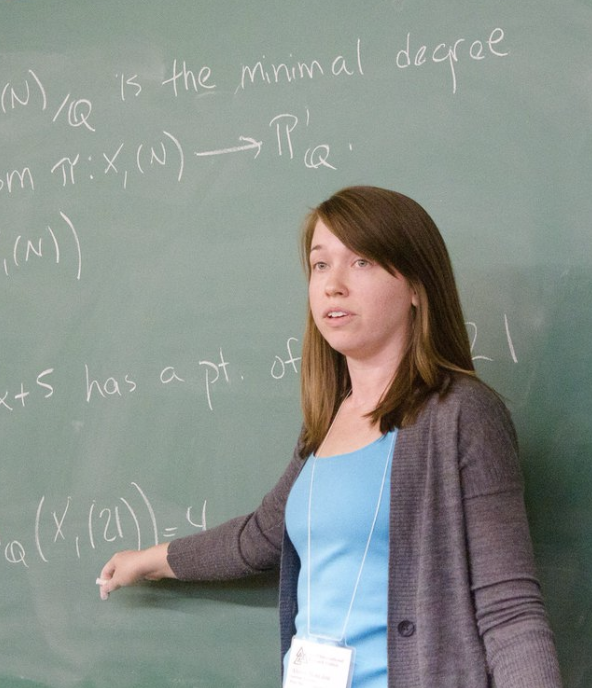
\includegraphics[width=0.65\textwidth]{images/bourdon.png}}
	\caption{\scriptsize Abbey Bourdon}
	\end{subfigure}
	%
	\begin{subfigure}{0.30\textwidth}
	\captionsetup{labelformat=empty}
	\centering
	\fbox{
\includegraphics[width=0.56\textwidth]{images/clark.jpg}}
	\caption{\scriptsize Pete Clark}
	\end{subfigure}
	%
	\begin{subfigure}{0.30\textwidth}
	\captionsetup{labelformat=empty}
	\centering
	\fbox{
\includegraphics[width=0.53\textwidth]{images/stankewicz.png}}
	\caption{\scriptsize James Stankewicz}
	\end{subfigure}
	\end{figure}
\end{frame}





% CM Bourdon Pollack
\begin{frame}[plain]
	\begin{thm}[Bourdon, Pollack; 2018]
	Let $K$ be an odd degree number field and $E/K$ be an elliptic curve with CM. Then the torsion subgroups $E(K)_\tors$ are computable. 
	\end{thm} 
	\begin{figure}[h]
	\centering
	\begin{subfigure}{0.3\textwidth}
	\captionsetup{labelformat=empty}
	\centering
	\fbox{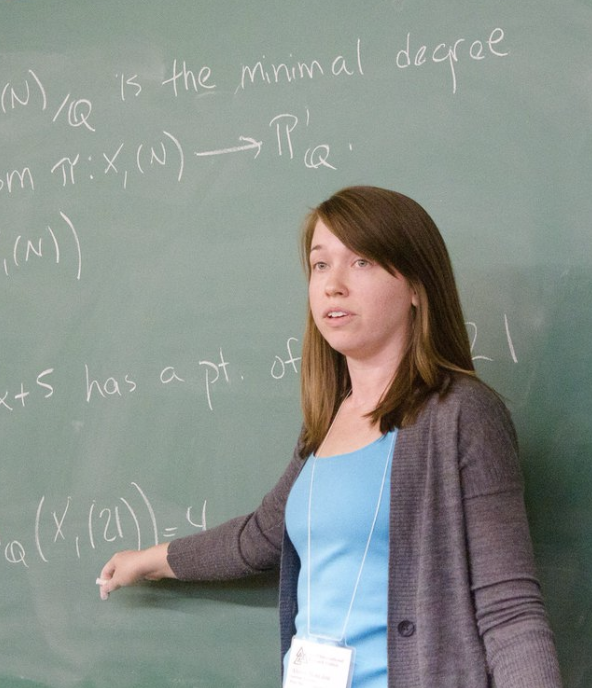
\includegraphics[width=0.85\textwidth]{images/bourdon.png}}
	\caption{Abbey Bourdon}
	\end{subfigure}
	%
	\begin{subfigure}{0.3\textwidth}
	\captionsetup{labelformat=empty}
	\centering
	\fbox{\includegraphics[width=0.82\textwidth]{images/pollack.jpg}}
	\caption{Paul Pollack}
	\end{subfigure}
	\end{figure}
\end{frame}



% CM Bourdon Pollack
\begin{frame}[plain]
\tiny
\begin{thm}[Bourdon, Chaos; 2022]
Let $F$ be a number field of degree $2p$ for $p > 5$ prime, and let $E/F$ be an elliptic curve with CM by the order of discriminant $\Delta$. Then $E(F)_\tors$ is new if and only if one of the following occurs:
	\begin{enumerate}[(i)]
	\item $\Delta= -115$, $p= 11$, and $E(F)_\tors \cong \Z/23\Z$, or 
	\item $\Delta= -235$, $p= 23$, and $E(F)_\tors \cong \Z/47\Z$, or
	\item $\Delta= \in \{ -11, -19, -27, -43, -67, -163 \}$, $p$ is a Germain prime with $\left( \dfrac{\Delta}{2p + 1} \right)= 1$, and $E(F)_\tors \cong \Z/(2p + 1)\Z$, or
	\item $\Delta \in \{ -8, -12, -16, -28 \}$, $p$ is a Germain prime with $\left( \dfrac{\Delta}{2p + 1} \right)= 1$, and $E(F)_\tors \cong \Z/2(2p + 1)\Z$, or 
	\item $\Delta= -7$, $p$ is a Germain prime with $\left( \dfrac{\Delta}{2p + 1} \right)= 1$, and $E(F)_\tors \cong \Z/2\Z \oplus \Z 2(2p + 1)\Z$, or
	\item $\Delta= -3$, $p= 7$, and $E(F)_\tors \cong \Z/49\Z$, or 
	\item $\Delta= -3$, $6p + 1$ is prime, and $E(F)_\tors \cong \Z/(6p + 1)\Z$, or
	\item $\Delta= -4$, $4p + 1$ is prime, and $E(F)_\tors \cong \Z/2(4p + 1)\Z$. 
	\end{enumerate}
In particular, any new torsion subgroup arises on one of only finitely many CM elliptic curves, and all but $\Delta= -115$ and $-235$ correspond to imaginary quadratic orders of class number 1. 
\end{thm} 

	\begin{figure}[h]
	\centering
	\begin{subfigure}{0.3\textwidth}
	\captionsetup{labelformat=empty}
	\centering
	\fbox{\includegraphics[width=0.59\textwidth]{images/bourdon.png}}
	\caption{\scriptsize Abbey Bourdon}
	\end{subfigure}
	%
	\begin{subfigure}{0.3\textwidth}
	\captionsetup{labelformat=empty}
	\centering
	\fbox{\includegraphics[width=0.465\textwidth]{images/chaos.jpeg}}
	\caption{\scriptsize Holly Paige Chaos}
	\end{subfigure}
	\end{figure}
\end{frame}



% Infinite Extensions
\begin{frame}[plain]
\ctext{Torsion over Infinite Extensions}
\end{frame}



% Maximal 2-Abelian
\begin{frame}[plain]
\footnotesize
\begin{thm}[Laska, Lorenz, 1985; Fujita, 2005]
Let $E/\Q$ be a rational elliptic curve, and let $\Q(2^\infty)$ be the maximal abelian 2-extension of $\Q$. Then $E(K)_\tors$ is isomorphic to precisely one of the following groups:
	\[
	\begin{cases}
	\Z/n\Z, & \text{with } n= 1, 3, 5, 7, 9, 15 \text{ or} \\
	\Z/2\Z \oplus \Z/2n\Z, & \text{with } n= 1, 2, 3, 4, 5, 6, 8 \text{ or} \\
	\Z/3\Z \oplus \Z/3\Z, & \text{ or} \\
	\Z/4\Z \oplus \Z/4n\Z, & \text{with } n= 1, 2, 3, 4 \text{ or} \\
	\Z/2n\Z \oplus \Z/2n\Z, & \text{with } n= 3, 4
	\end{cases}
	\]
and each such possibility occurs. 
\end{thm}
	\begin{figure}[h]
	\centering
	\begin{subfigure}{0.30\textwidth}
	\captionsetup{labelformat=empty}
	\centering
	\fbox{\includegraphics[width=0.42\textwidth]{images/laska.png}}
	\caption{\scriptsize Michael Laska}
	\end{subfigure}
	%
	\begin{subfigure}{0.30\textwidth}
	\captionsetup{labelformat=empty}
	\centering
	\fbox{\includegraphics[width=0.46\textwidth]{images/lorenz.jpeg}}
	\caption{\scriptsize Martin Lorenz}
	\end{subfigure}
	%
	\begin{subfigure}{0.30\textwidth}
	\captionsetup{labelformat=empty}
	\centering
	\fbox{\includegraphics[width=0.47\textwidth]{images/fujita.png}}
	\caption{\scriptsize Yasutsugu Fujita}
	\end{subfigure}
	\end{figure}
\end{frame}



% Maximal 3-Abelian
\begin{frame}[plain]
\footnotesize
\begin{thm}[Daniels, Lozano-Robledo, Najman, Sutherland, 2017]
Let $E/\Q$ be a rational elliptic curve. Then the torsion subgroup $E(\Q(3^\infty))_\tors$ is finite and is isomorphic to precisely one of the following groups:
	\[
	\begin{cases}
	\Z/2\Z \oplus \Z/2n\Z, & \text{with } n= 1, 2, 4, 5, 7, 8, 13 \text{ or} \\
	\Z/4\Z \oplus \Z/4n\Z, & \text{with } n= 1, 2, 4, 7 \text{ or} \\
	\Z/6\Z \oplus \Z/6n\Z, & \text{with } n= 1, 2, 3, 5, 7 \text{ or} \\
	\Z/2n\Z \oplus \Z/2n\Z, & \text{with } n= 4, 6, 7, 9. \\
	\end{cases}
	\]
All but four of the torsion subgroups, $T$, listed above occur for infinitely many $\ov{\Q}$-isomorphism classes of elliptic curves $E/\Q$. For $T \cong \Z/4\Z \oplus \Z/28\Z$, $\Z/6\Z \oplus \Z/30\Z$, $\Z/6\Z \oplus \Z/42\Z$, and $\Z/14\Z \oplus \Z/14\Z$, there are only 2, 2, 4, and 1 (respectively) $\ov{\Q}$-isomorphism classes of $E/\Q$ for which $E(\Q(3^\infty))_\tors \cong T$. 
\end{thm}
	\begin{figure}[h]
	\centering
	\begin{subfigure}{0.23\textwidth}
	\captionsetup{labelformat=empty}
	\centering
	\fbox{\includegraphics[width=0.85\textwidth]{images/daniels.jpeg}}
	\caption{\scriptsize Harris Daniels}
	\end{subfigure}
	%
	\begin{subfigure}{0.23\textwidth}
	\captionsetup{labelformat=empty}
	\centering
	\fbox{\includegraphics[width=0.72\textwidth]{images/lozano.jpeg}}
	\caption{\scriptsize \hspace{0.70cm}\'Alvaro \\ \;\;Lozano-Robledo}
	\end{subfigure}
	%
	\begin{subfigure}{0.23\textwidth}
	\captionsetup{labelformat=empty}
	\centering
	\fbox{\includegraphics[width=0.60\textwidth]{images/najman2.png}}
	\caption{\scriptsize Filip Najman}
	\end{subfigure}
	%
	\begin{subfigure}{0.23\textwidth}
	\captionsetup{labelformat=empty}
	\centering
	\fbox{\includegraphics[width=0.77\textwidth]{images/sutherland.jpg}}
	\caption{\scriptsize Andrew Sutherland}
	\end{subfigure}
	\end{figure}
\end{frame}



% D4 Extensions
\begin{frame}[plain]
\footnotesize
\begin{thm}[Daniels, 2017]
Let $E/\Q$ be a rational elliptic curve. Then $E(\Q(D_4^\infty))$ is finite and isomorphic to one of the following:
	\[
	\begin{cases}
	\Z/n\Z, & \text{with } n= 1, 3, 5, 7, 9, 13, 15 \text{ or} \\
	\Z/3\Z \oplus \Z/3n\Z, & \text{with } n= 1, 5 \text{ or} \\
	\Z/4\Z \oplus \Z/4n\Z, & \text{with } n= 1, 2, \ldots, 6, 8 \text{ or} \\
	\Z/8\Z \oplus \Z/8n\Z, & \text{with } n= 1, 2, 3, 4 \text{ or} \\
	\Z/12\Z \oplus \Z/12n\Z, & \text{with } n= 1, 2 \text{ or} \\
	\Z/n\Z \oplus \Z/n\Z, & \text{with } n= 5, 16.
	\end{cases}
	\]
All but 3 of the 24 torsion structures listed above occur for infinitely many $\overline{\Q}$-isomorphism classes of elliptic curves $E/\Q$. The torsion structures that occur finitely often are $\Z/15\Z$, $\Z/3\Z \oplus \Z/15\Z$, and $\Z/12\Z \oplus \Z/12\Z$, which occur for 4, 2, and 1 $\overline{\Q}$-isomorphism classes, respectively. 
\end{thm}
	\begin{figure}[!ht]
	\centering
	\captionsetup{labelformat=empty}
	\fbox{\includegraphics[width=0.18\textwidth]{images/daniels.jpeg}}
	\caption{\scriptsize Harris Daniels}
	\end{figure}
\end{frame}



% A4
\begin{frame}[plain]
\footnotesize
\begin{thm}[Daniels, Derickx, Hatley, 2019]
Let $E/\Q$ be an elliptic curve. The torsion subgroup $E(\Q(A_4^\infty))_\tors$ is finite and isomorphic to one of the following:
	\[
	\begin{cases}
	\Z/n\Z, & \text{with } n= 1, 3, 5, 7, 9, 13, 15, 21 \text{ or} \\
	\Z/2\Z \oplus \Z/2n\Z, & \text{with } n= 1, 2, \ldots, 9 \text{ or} \\
	\Z/3\Z \oplus \Z/3n\Z, & \text{with } n= 1, 3 \text{ or} \\
	\Z/4\Z \oplus \Z/4n\Z, & \text{with } n= 1, 2, 3, 4, 7 \text{ or} \\
	\Z/n\Z \oplus \Z/n\Z, & \text{with } n= 6, 8.
	\end{cases}
	\]
All but 4 of the 26 torsion structures listed above occur for infinitely many $\overline{\Q}$-isomorphism classes of elliptic curves $E/\Q$. The torsion structures that occur finitely often are $\Z/21\Z$, $\Z/15$, $\Z/2\Z \oplus \Z/14\Z$, and $\Z/3\Z \oplus \Z/9\Z$, which occur for 4, 2, 2, and 1 $\overline{\Q}$-isomorphism classes, respectively.  
\end{thm}
	\begin{figure}[h]
	\centering
	\begin{subfigure}{0.30\textwidth}
	\captionsetup{labelformat=empty}
	\centering
	\fbox{\includegraphics[width=0.65\textwidth]{images/daniels.jpeg}}
	\caption{\scriptsize Harris Daniels}
	\end{subfigure}
	%
	\begin{subfigure}{0.30\textwidth}
	\captionsetup{labelformat=empty}
	\centering
	\fbox{\includegraphics[width=0.52\textwidth]{images/derickx.jpg}}
	\caption{\scriptsize Maarten Derickx}
	\end{subfigure}
	%
	\begin{subfigure}{0.30\textwidth}
	\captionsetup{labelformat=empty}
	\centering
	\fbox{\includegraphics[width=0.70\textwidth]{images/hatley.png}}
	\caption{\scriptsize Jeffrey Hatley}
	\end{subfigure}
	\end{figure}
\end{frame}



% Maximal Abelian Extension
\begin{frame}[plain]
\scriptsize
\begin{thm}[Chou, 2019]
Let $E/\Q$ be a rational elliptic curve. Then $E(\Q^{\text{ab}})_\tors$ is finite, and is isomorphic to precisely one of the following groups:
	\[
	\begin{cases}
	\Z/n\Z, & \text{with } n= 1, 3, 5, 7, 9, 11, 13, 15, 17, 19, 21, 25, 27, 37, 43, 67, 163 \text{ or} \\
	\Z/2\Z \oplus \Z/2n\Z, & \text{with } n= 1, 2, \ldots, 9 \text{ or} \\
	\Z3\Z \oplus \Z/3n\Z, & \text{with } n= 1, 3 \text{ or} \\
	\Z/4\Z \oplus \Z/4n\Z, & \text{with } n= 1, 2, 3, 4 \text{ or} \\
	\Z/n\Z \oplus \Z/n\Z, & \text{with } n= 5, 6, 8.
	\end{cases}
	\]
Each of the listed groups appears as a torsion subgroup for $E(\Q^{\text{ab}})_\tors$ for some elliptic curve over $\Q$. 
\end{thm}
	\begin{figure}[!ht]
	\centering
	\captionsetup{labelformat=empty}
	\fbox{\includegraphics[width=0.20\textwidth]{images/chou.jpg}}
	\caption{Michael Chou}
	\end{figure}
\end{frame}



% Zp Extensions
\begin{frame}[plain]
\footnotesize
\begin{thm}[Chou, Daniels, Krijan, Najman, 2018]
Let $p$ be a prime, and let $E/\Q$ be an elliptic curve. Then if $p= 2, 3$, then $E(\Q_{\infty, p})_\tors$ is one of the following groups:
	\[
	\begin{cases}
	\Z/n\Z, & n= 1, 2, \ldots, 10, 12, 21^*, 27^* \text{ or} \\
	\Z/2\Z \oplus \Z/2n\Z, & n= 1, 2, 3, 4, \\
	\end{cases}
	\]
where the starred cases can only occur if $p= 3$. If $p \neq 2, 3$, then $E(\Q_{\infty, p})_\tors=$ $E(\Q)_\tors$. Each of the groups listed above appears as a torsion subgroup for $E(\Q_{\infty,p})_\tors$ for some $E/\Q$ and each $p$ possible.
\end{thm}

	\begin{figure}[h]
	\centering
	\begin{subfigure}{0.23\textwidth}
	\captionsetup{labelformat=empty}
	\centering
	\fbox{\includegraphics[width=0.64\textwidth]{images/chou.jpg}}
	\caption{\scriptsize Michael Chou}
	\end{subfigure}
	%
	\begin{subfigure}{0.23\textwidth}
	\captionsetup{labelformat=empty}
	\centering
	\fbox{\includegraphics[width=0.85\textwidth]{images/daniels.jpeg}}
	\caption{\scriptsize Harris Daniels}
	\end{subfigure}
	%
	\begin{subfigure}{0.23\textwidth}
	\captionsetup{labelformat=empty}
	\centering
	\fbox{\includegraphics[width=0.64\textwidth]{images/krijan.jpeg}}
	\caption{\scriptsize Ivan Krijan}
	\end{subfigure}
	%
	\begin{subfigure}{0.23\textwidth}
	\captionsetup{labelformat=empty}
	\centering
	\fbox{\includegraphics[width=0.60\textwidth]{images/najman2.png}}
	\caption{\scriptsize Filip Najman}
	\end{subfigure}
	\end{figure}
\end{frame}



% Zp Other
\begin{frame}[plain]
\scriptsize
\begin{thm}[Gu{\u{z}}vi\'c, Vukorepa, 2022]
Let $E/\Q$ be an elliptic curve. Then $E(\Q(\zeta_{16}))_\tors \in \Phi(1)$ or is one of $\Z/4\Z \oplus \Z/4\Z$, $\Z/2\Z \oplus \Z/10\Z$ and $E(\Q(\zeta_{27}))_\tors \in \Phi(1)$ or is one of $\Z/3\Z \oplus \Z/3n\Z$ with $n= 1, 2, 3$, $\Z/21\Z$, or $\Z/27\Z$. Furthermore, let $p \in \{5, 7, 11 \}$. Then either $E(\Q(\zeta_p))_\tors \in \Phi(1)$ or is one of $\Z/5\Z \oplus \Z/5\Z$, $\Z/15\Z$, or $\Z/16\Z$, if $p= 5$, or $\Z/n\Z$ with $n= 13, 14, 18$ or $\Z/2\Z \oplus \Z/2n\Z$ with $n= 7, 9$, if $p= 7$, or $\Z/11\Z$, $\Z/25\Z$, or $\Z/2\Z \oplus \Z/10\Z$, if $p= 11$. 
\end{thm}

\begin{thm}[Gu{\u{z}}vi\'c, Krijan, 2020]
Let $\mathcal{K}= \prod_{p \text{ prime}} \Q_{\infty, p}$ and $\mathcal{K}_{\geq p}= \prod_{q \text{ prime}, q \geq p}$, and let $E/\Q$ be an elliptic curve. Then $E(\mathcal{K}_{\geq 5})_\tors= E(\Q)_\tors$ and $E(\mathcal{K})_\tors$ is isomorphic to precisely one of the following:
	\[
	\begin{cases}
	\Z/n\Z, & \text{with } n= 1, 2, \ldots, 10, 12, 13, 21, 27 \text{ or} \\
	\Z/2\Z \oplus \Z/2n\Z, & \text{with } n= 1, 2, 3, 4. \\
	\end{cases}
	\]
Moreover, each such group above occurs for some elliptic curve $E/\Q$. 
\end{thm}

	\begin{figure}[h]
	\centering
	\begin{subfigure}{0.23\textwidth}
	\captionsetup{labelformat=empty}
	\centering
	\fbox{\includegraphics[width=0.72\textwidth]{images/guzvic2.jpg}}
	\caption{\scriptsize Tomislav Gu{\u{z}}vi\'c}
	\end{subfigure}
	%
	\begin{subfigure}{0.23\textwidth}
	\captionsetup{labelformat=empty}
	\centering
	\fbox{\includegraphics[width=0.65\textwidth]{images/krijan.jpeg}}
	\caption{\scriptsize Ivan Krijan}
	\end{subfigure}
	%
	\begin{subfigure}{0.30\textwidth}
	\captionsetup{labelformat=empty}
	\centering
	\fbox{\includegraphics[width=0.50\textwidth]{images/vukorepa.jpeg}}
	\caption{\scriptsize Borna Vukorepa}
	\end{subfigure}
	\end{figure}
\end{frame}



% 2-adic
\begin{frame}[plain] \footnotesize
\begin{thm}[Rouse,Zureick-Brown, 2015]
Let $E/\Q$ be a rational elliptic curve without CM. Then the index of $\rho_{E,2^\infty}(\Gal(\overline{\Q}/Q))$ divides 64 or 96, and all such indices occur. Furthermore, the image of $\rho_{E,2^\infty}(\Gal(\overline{\Q}/\Q))$ is the inverse image in $\GL_2(\Z_2)$ of the image of $\rho_{E,32}(\Gal(\overline{\Q}/\Q))$.
\end{thm}
	\begin{figure}[h]
	\centering
	\begin{subfigure}{0.3\textwidth}
	\captionsetup{labelformat=empty}
	\centering
	\fbox{\includegraphics[width=0.70\textwidth]{images/rouse.jpg}}
	\caption{Jeremy Rouse}
	\end{subfigure}
	%
	\begin{subfigure}{0.3\textwidth}
	\captionsetup{labelformat=empty}
	\centering
	\fbox{\includegraphics[width=0.69\textwidth]{images/zbrown.png}}
	\caption{David Zureick-Brown}
	\end{subfigure}
	\end{figure}
\begin{rem}
They also enumerate all 1,208 possibilities and find their rational points. 
\end{rem}
\end{frame}



% Zwyina
\begin{frame}[plain]
\begin{thm}[Sutherland, Zywina, 2016]
Up to conjugacy, there are 248 open subgroups of $\GL_2(\hat{\Z})$ of prime power level satisfying $-I \in G$ and $\det G= \hat{\Z}^\times$ for which $X_G$ has infinitely many rational points. Of these 248 groups, there are 220 of genus 0 and 28 of genus 1. 
\end{thm}
	\begin{figure}[h]
	\centering
	\begin{subfigure}{0.3\textwidth}
	\captionsetup{labelformat=empty}
	\centering
	\fbox{\includegraphics[width=0.82\textwidth]{images/sutherland.jpg}}
	\caption{Drew Sutherland}
	\end{subfigure}
	%
	\begin{subfigure}{0.3\textwidth}
	\captionsetup{labelformat=empty}
	\centering
	\fbox{\includegraphics[width=0.77\textwidth]{images/zwyina.jpg}}
	\caption{\hspace{0.1cm}David Zywina}
	\end{subfigure}
	\end{figure}
\end{frame}



% Possible Prime Divisors
\begin{frame}[plain]
\ctext{Possible Prime Divisors}
\end{frame}



% S_Q(d)
\begin{frame}[plain]
	\begin{thm}[Mazur, Parent, Derickx, Kammienny, Stein, Stoll, Lozano-Robledo, et al.]
		\[
		\begin{split}
		S_\Q(\{1,2\})&= \{ 2,3,5,7 \} \\
		S_\Q(\{3,4\})&= \{ 2,3,5,7,13 \} \\
		S_\Q(\{5,6,7\})&= \{ 2,3,5,7,11,13 \} \\
		S_\Q(8)&= \{ 2,3,5,7,11,13 \} \\
		S_\Q(\{9,10,11\})&= \{ 2,3,5,7,11,13,17,19 \} \\
		S_\Q(\{12,\ldots,20\})&= \{2,3,5,7,11,13,17,19,37 \} \\
		S_\Q(21)&= \{ 2,3,5,7,11,13,17,19,37,43 \}
		\end{split}
		\]
	\end{thm}
\end{frame}



% Serre
\begin{frame}[plain]
\begin{rem}
Lozano-Robledo computes $S_\Q(d)$ for $1 \leq d \leq 21$, and gives a conjecturally formula valid for all $1 \leq d \leq 42$, following from a positive answer to Serre's uniformity question.
\end{rem}
	\begin{figure}[h]
	\centering
	\begin{subfigure}{\textwidth}
	\captionsetup{labelformat=empty}
	\centering
	\fbox{\includegraphics[width=0.25\textwidth]{images/robledo.jpg}}
	\caption{\'Alvaro Lozano-Robledo}
	\end{subfigure}
	\end{figure}
\begin{rem}
Furthermore, Enrique Gonz\'alez-Jim\'enez and Filip Najman determine all possible prime orders of a point $P \in E(K)_\tors$, where $[K : \Q]= d$ for all $d \leq 3\,342\,296$.
\end{rem}
\end{frame}



% Min Field
\begin{frame}[plain]
\begin{thm}[Gonz\'alez-Jim\'enez, Lozano-Robledo, 2015]
Let $E/\Q$ be an elliptic curve without CM. Let $1 \leq s \leq N$ be fixed integers, and let $T \subseteq E[2^N]$ be a subgroup isomorphic to $\Z/2^s/Z \oplus \Z/2^N \Z$. Then $[\Q(T) \colon \Q]$ is divisible by 2 if $s=N=2$, and otherwise by $2^{2N+2s-8}$ if $N \geq 3$, unless $s \geq 4$ and $j(E)$ is one of the two values:
	\[
	- \dfrac{3 \cdot 18249920^3}{17^{16}}\; \text{ or } - \dfrac{7 \cdot 1723187806080^3}{79^{16}}
	\]
in which case $[\Q(T) \colon \Q]$ is divisible by $3 \cdot 2^{2N+2s-9}$. Moreover, this is best possible in that there are one-parameter families $E_{s,N}(t)$ of elliptic curves over $\Q$ such that for each $s, N \geq 0$ and each $t \in \Q$, and subgroups $T_{s,N} \in E_{s,N}(t)(\ov{\Q})$ isomorphic to $\Z/2^s\Z \oplus \Z/2^N\Z$ such that $[\Q(T_{s,N}) \colon \Q]$ is equal to the bound given above. 
\end{thm}
\end{frame}



% Functions Fields
\begin{frame}[plain]
\ctext{Torsion over Function Fields}
\end{frame}



% McDonald
\begin{frame}[plain]
\begin{thm}[McDonald, 2017]
Let $K= \F_q(T)$, where $q=p^n$. Let $E/K$ be non-isotrivial. If $p \nmid E(K)_\tors$, then $E(K)_\tors$ is one of the following: $0,\Z/2\Z, \ldots,\Z/10\Z,\Z/12\Z, \Z/2\Z \oplus \Z/2\Z, \Z/2\Z \oplus \Z/4\Z, \Z/2\Z \oplus \Z/6\Z, \Z/2\Z \oplus \Z/8\Z, \Z/3\Z \oplus \Z/3\Z, \Z/3\Z \oplus \Z/6\Z, \Z/4\Z \oplus \Z/4\Z, \Z/5\Z \oplus \Z/5\Z$.

If $p \mid \#E(K)_\tors$, then $p \leq 11$, and $E(K)_\tors$ is one of
	\[
	\begin{cases}
	\Z/p\Z, & p=2,3,5,7,11 \\
	\Z/2p\Z, & p=2,3,5,7 \\
	\Z/3p\Z, & p=2,3,5 \\
	\Z/4p\Z, & p=2,3 \\
	\Z/5p\Z, & p=2,3 \\
	\Z/5\Z \oplus \Z/10\Z, & p=2 \\
	\Z/2\Z \oplus \Z/12\Z, & p=3 \\
	\Z/2\Z \oplus \Z/10\Z, & p=5
	\end{cases}
	\]
\end{thm}
\end{frame}


% McDonald
\begin{frame}[plain]
\ctext{
	\begin{figure}
	\captionsetup{labelformat=empty}
	\centering
	\fbox{\includegraphics[width=0.30\textwidth]{images/mcdonald.jpg}}
	\caption{Robert McDonald}
	\end{figure}
}
\end{frame}